
\documentclass[a4paper,11pt]{book}

%%%%%%%%%
%%uses%%
%%%%%%%%%
\usepackage[utf8]{inputenc}
%\usepackage[ngerman]{babel}
%\usepackage{a4wide}
\usepackage[margin=3.0cm, top=3.0cm, bottom=3.0cm]{geometry}
\usepackage{setspace}
\usepackage{graphicx}
\usepackage{amssymb} 
\usepackage{amsmath}
\usepackage{mathtools}
\usepackage{footnote}
\usepackage{caption}
\usepackage{subcaption}
\usepackage{color}
\usepackage[hidelinks]{hyperref}
\usepackage{cite}
\usepackage{setspace}



%%%%%%%%%
%%Title%%
%%%%%%%%%

\author{Frederik Zwilling 304314}
\title{Simulation of the RoboCup Logistic League with Fawkes and Gazebo for Multi-Robot Coordination Evaluation}
\begin{document}
\begin{titlepage}
  
  \begin{center}
    
    \Large
    \textsc{Rheinisch-Westfälische Technische Hochschule Aachen}\\
    Knowledge-Based Systems Group\\
    Prof. G. Lakemeyer, Ph.D.\\
    
    \vspace{4cm}
    

    \hrule \\
    [0.4cm]
           {
             \Huge 
             \bfseries
             Simulation of the RoboCup Logistic League with Fawkes and Gazebo for Multi-Robot Coordination Evaluation\\
           }\\
   [0.4cm]
   \hline \\
   [1.5cm]
   
    \textsc{Bachelor-Thesis}\\
    by\\ 
    [0.4cm]
    \large Frederik Zwilling\\
    \normalsize
    Matrikelnummer: 304314\\
    frederik.zwilling@rwth-aachen.de\\

    \vspace{8cm}
    
    \today
  \end{center}

\end{titlepage}

\newpage
\thispagestyle{empty}
\mbox{}
 \newpage
\Large
\begin{tabular}{ l l }
First Supervisor: & Prof. Gerhard Lakemeyer, Ph.D.\\
\\
Second Supervisor: & Prof. Dr. Matthias Jarke\\
\\
Advisor: &  Dipl. Inform. Tim Niemueller\\
\end{tabular}

\vspace{7cm}
Hiermit versichere ich, dass ich die Arbeit selbststandig verfasst und keine anderen als die angegebenen Quellen und Hilfsmittel verwendet sowie Zitate kenntlich gemacht habe.\\

\vspace{3cm}

\large
\makebox[2.5in]{\hrulefill} \hspace {1.0in} \makebox[2.5in]{\hrulefill} \\
\makebox[2.5in]{Place, Date} \hspace {1.0in} \makebox[2.5in]{Signature (Frederik Zwilling)} \\
\normalsize

 \frontmatter
\newpage

\section*{Acknowledgements}

I would like to thank Tim Niem\"{u}ller and Professor Lakemeyer for the opportunity to work on the amazing field of robot software and for their valuable support.\\
For a very fascinating and exciting time with great teamwork, I also want to thank the Carologistics team, especially Tim Niem\"{u}ller, Sebastian Reuter, Daniel Ewert, Victor Matar\'{e}, Florian Nolden, Tobias Neumann, Johannes Rothe, Bahram Maleki-Fard, Andre Burghof, Professor Ferrein, Professor Lakemeyer and Professor Jeschke.\\
I am very grateful to Julia Karoline Karrenbrock for her support and patience in all those months. I would also like to thank my family and friends for their support and patience.

\newpage
\tableofcontents
\newpage
\listoffigures
\listoftables
\newpage
\onehalfspace
\mainmatter

%%%%%%%%%
%%Text%%
%%%%%%%%

%\abstract{This is the abstract.}

%avoid empty pages before chapter
\let\cleardoublepage\clearpage

\chapter{Introduction}

Multi-robot systems are combinations of multiple robots that are made to work together on specific tasks. Currently, they are mostly used in assembly lines, where many robot-arms simultaneously do repetitive tasks with the same object. More autonomous examples of multi-robot systems can be found in the warehousing domain. Here, many robots bring demanded goods and store new ones~\cite{Kiva}. The major advantages of multi-robot systems are high flexibility and the possibility to run different tasks in parallel. The amount of possible applications is large. Besides assembly and warehousing, they also can be used in rescue scenarios~\cite{mas_rescue}, soccer~\cite{mas_soccer}, planetary exploration~\cite{mas_space}, logistics and more.\\
Developing a robotic system is challenging. Robots have to detect objects, localize themselves, reason about their surrounding and manipulate it. Developing a multi-robot system is even harder because the robots have to do all this in coordination with other robots. Furthermore the systems have to be robust against the failure of single robots and should be as efficient as possible. Because of these challenges, testing is an essential part of the development process. It is necessary to identify mistakes in the source code and to evaluate how the system performs in a complex environment. Often, tests reveal problems the developer has not expected. However, testing can be difficult and time consuming. The robot and the environment have to be available and set up. A component to test can depend on other components that are still in development. Some tests require cautious execution because the robot could harm itself or the environment and full system tests have to run a longer time. Testing a multi-robot system is even harder. On the one hand the testing effort scales with the number of robots. On the other hand the system is more complex and therefore requires more test runs for evaluation.\\
In this thesis we tackle these problems by developing a multi-robot simulation environment. We simulate multiple robots in a physically and visually realistic three-dimensional environment. The robot software runs as in the real world and gets simulated sensor data instead of real sensor data. When the robot software uses actuators, the actions are executed in the simulation. This brings many advanteges and can speed up the testing process. With a simulation environment, the majority of tests does not need available robots and the environment, the setup can be automated, unfinished components other components depend on can be simulated as well. Furthermore we want to evaluate the whole multi-robot system by measuring its performance in multiple runs. This makes us able to easily compare different configurations and strategies in the simulation.\\
Such a simulation is usefull in most robot developments. In this thesis we concentrate on the logistics domain and the mobile robot platform \textit{Robotino}. We participate with the \textit{Carologistics} team in the \textit{Logistic Leage sponsored by Festo (LLSF)}. The Carologistics is a joint team consisting of the Knowledge-based Systems Group at RWTH Aachen University, the IMA/ZLW \& IFU Institute Cluster at RWTH Aachen University and the Department for Electrical Engineering and Information Technology, Robotics Group at FH Aachen. LLSF is an industrial motivated competition within the RoboCup initiative. Three robots have to manage the material flow in a production area. The goal is to produce as many ordered products by feeding different machines in the production area with ressources and intermediate products. To achieve a good performance, robust robot behavior and an efficient scheduling is necessary. Because of this, we have a special need for a multi-robot simulator, which can test the performance of single robots as well as the efficency of the whole multi-robot system.\\
We use the \textit{Fawkes} robot software framework to control the robots and we have choosen \textit{Gazebo} as robot simulator. Important task of this thesis are the connection between Fawkes and Gazebo, the simulation of sensor data and the modeling of LLSF environment and the robots actions in this environment. Because we want to use the multi-robot simulation to evaluate and improve our own LLSF system, we will also develop some concrete improvements and compare the perfomances of the system with different configurations. The majority of these improvements relate to the high level agent, which is responsible for the decisions of the robot and the coordination between the agents.
\\
In chapter 2, we show the background of this thesis. This includes descriptions of the Robotino, the RoboCup and LLSF, Fawkes, Gazebo and the current LLSF solution of the Carologistics team. In chapter 3, we present related work about other simulations and agent strategies. The design ideas and thoughts behind the simulation are described in chapter 4. In chapter 5, we present the implementation. This includes general usage of the used tools, a description of the developed simulation modules and the improvements on our LLSF system. The evaluation-results of the agent changes and the simulation itself are shown in chapter 6. In chapter 7, we suggest future work and conclude in chapter 8.

\section{Background}

This is the background.

\chapter{Related Work}
\label{cha:related_work}
In this chapter we present work related to this thesis. In section~\ref{sec:other_simulators}, we describe alternatives to Gazebo and why we choose Gazebo. In section~\ref{sec:simulations}, we give an overview of other popular simulations, especially a simulation that also uses Gazebo and other multi-robot simulations, and in section~\ref{sec:multi_agent_strategies}, we describe our current multi-robot strategy as well as other attractive strategies our simulation should be able to evaluate. In the following, we will use the terms \textit{multi-robot} and \textit{multi-agent} interchangeably because the common term in literature is multi-agent and we want to use multi-robot. A multi-agent system can consist of fully abstract agents, such as \textcolor{red}{...}, whereas we are dealing with multi-robot system and therefore robots that interact physically with their environment.


\section{Other Simulators}
\label{sec:other_simulators}
\textcolor{red}{blabla?}
\subsection{Stage}
\textit{Stage}\footnote{\url{http://playerstage.sourceforge.net/index.php?src=stage}} is an Open Source multi-robot simulator for a two dimensional environment. It is a part of the \textit{Player/Stage} project~\cite{{PlayerStage}}. \textit{Player} is a robot control server, which provides a simple connection between a robot control program and the sensors and actuators of a robot. Stage uses this connection and replaces the sensors and actuators by simulated ones. Stage was popular simulator in the last years and is able to simulate a large amount of robots. For the simulation, stages simple and computationally cheap models, that provide still enough fidelity for most applications. Furthermore the computational effort is linear in the number of robots. Because of that, Stage can simulate large amounts of robots~\cite{stage_massive}. This makes Stage attractive for the simulation of swarms and multi-robot systems with many robots.

\subsection{Webots}
\textit{Webots}\footnote{\url{http://www.cyberbotics.com}} is a commercial 3D-simulator~\cite{{Webots}}. It is platform independent features a whole development environment for robot software including an editor and an \textcolor{red}{API} for inter-robot communication. Webots supports many programming languages and supports a variation of standard robots and sensors out of the box. It is also able to simulate multiple robots and provides a ROS and \textcolor{red}{Matlab} interface.\\
Webots was used in a RoboCup Soccer simulation league~\cite{webots_robocup}.

\subsection{USARSim}
\textit{USARSim} is a 3D-simulator that was developed for urban search and rescue scenarios~\cite{USARSim}. It was evolved to be able to simulate other domains too. Therefore, the abbreviation USARSim now stands for ``Unified System for Automation 
and Robotics Simulation'' instead of the previous ``Urban Search and Rescue Simulation''~\cite{usarsim_new}. It is platform independent and free of charge for research and education. It's advantages are the graphical quality of the Unreal engine\footnote{\url{http://www.unrealengine.com/udk}} and the PhysX physics engine\footnote{\url{https://developer.nvidia.com/physx}}. USARSim also provides an interface to ROS~\cite{USARSimROS} and is able to simulate multiple robots.\\
USARSim is used as a basis for the RoboCup Rescue Simulation League we also present in section 3.2.2.

\subsection{SimSpark}
\textit{SimSpark}\footnote{\url{http://simspark.sourceforge.net/}} is an Open Source 3D simulator~\cite{simspark_old}. It was developed by the RoboCup community for the RoboCup 3D Soccer Simulation and has been used there since 2004. Therefore SimSpark is able to simulate multiple robots and specialized on the NAO as soccer robot. There are several improvements and new features of SimSpark~\cite{SimSpark,Visualization}, such as visualization of agent-intentions, realistic servo motors for the NAO and better support of heterogeneous robot teams.

\subsection{Robotino Sim Professional}
\textit{Robotino Sim Professional}\footnote{\url{http://www.festo-didactic.com/int-en/learning-systems/software-e-learning/robotino-sim-view/robotino-sim-professional.htm}} is a 3D-simulator for the Robotino developed by its manufacturer Festo. It is a commercial software and only usable on Microsoft Windows. Furthermore, it is limited to the Robotino and the default sensors the Robotino is sold with.

\subsection{Choice for Gazebo}
We already presented Gazebo and some of its advantages in section 2.4. Here we explain why we have chosen Gazebo instead of an alternative we described above.\\
The stage simulator is well suited for multi-robot systems and comparatively fast and easy to use. However, the restriction to dimensions is a problem. We want to simulate vision components as well to be able to test our system as a whole and more realistic. We also want to be extendable for future changes of LLSF or the use of the simulator in an other domain, such as the RoboCup @Home league.\\
Webots is a proven simulator with many features, but has the same problems as Robotino Sim Professional. On the one hand both simulators are commercial and on the other hand both are no Open Source software. Therefore it can be difficult to expand the simulation how we need it.\\
SimSpark is not so well suited as Gazebo because it and the community behind are mostly specialized on the RoboCup Soccer Simulation. Gazebo is used in large variety of domains and has a bigger community. Gazebo is well founded by the Open Source Robotics Foundation\footnote{\url{http://osrfoundation.org/}} and Willow Garage\footnote{\url{http://www.willowgarage.com/}} and there are also many plans to develop Gazebo further\footnote{\textcolor{red}{link road-map}}. Therefore Gazebo is likely to become even more important in the future.\\
An other important argument for Gazebo is that it was used at KBSG before. It was used as a simulator for MSL~\cite{MultiLevelAbstraction} and it was used for a scene reconstruction~\cite{KlingenDA}. We will present both later in this chapter.\\
There are only few disadvantages of Gazebo for this thesis. A disadvantage is that Gazebo can not handle larger number of robots. The complexity of the simulations limits the simulation speed when using multiple robots. The number of robots to simulate at a reasonable speed is in the order of ten~\cite{GazeboDesign}. This can become a problem if the simulation runs on a slow computer or there are more robots to simulate at the same time.

\section{Simulations}
\label{sec:simulations}
\textcolor{red}{blabla?}
\subsection{Virtual Robotics Challenge}
The \textit{Virtual Robotics Challenge (VRC)} is a competition by DARPA\footnote{DARPA is the Defense Advanced Research Projects Agency of the USA.}. The goal of the competition is to solve challenging tasks with a humanoid robot in a simulation. VRC is the first part of the \textit{DARPA Robotics Challenge (DRC)}\footnote{\url{http://www.theroboticschallenge.org/}}. DRC aims to spur the development of robots that can operate in a disaster scenario if the situation is too dangerous for humans. An example for such a scenario is the disaster in the Fukushima nuclear power plant after tsunami in March 2011~\cite{fukushima}. The developed robots should be able to operate in environment made for humans, even if the environment is damaged, and to use tools made for humans, such as screwdrivers and cars. During the competition the robots act partly autonomously and are supervised by a human instructor. For the challenge, DARPA provides six humanoid robots. The Robots are called ATLAS and are developed by Boston Dynamics. The six best teams of VRC receive a ATLAS robot for free. Therefore ATLAS is the only robot simulated in VRC. However the participating teams can also build their own robots. VRC consists of three different tasks~\cite{vrc_rules} showed in Figure~\ref{fig:vrc}.
\begin{figure}
  \centering
  \begin{subfigure}[b]{0.3\textwidth}
    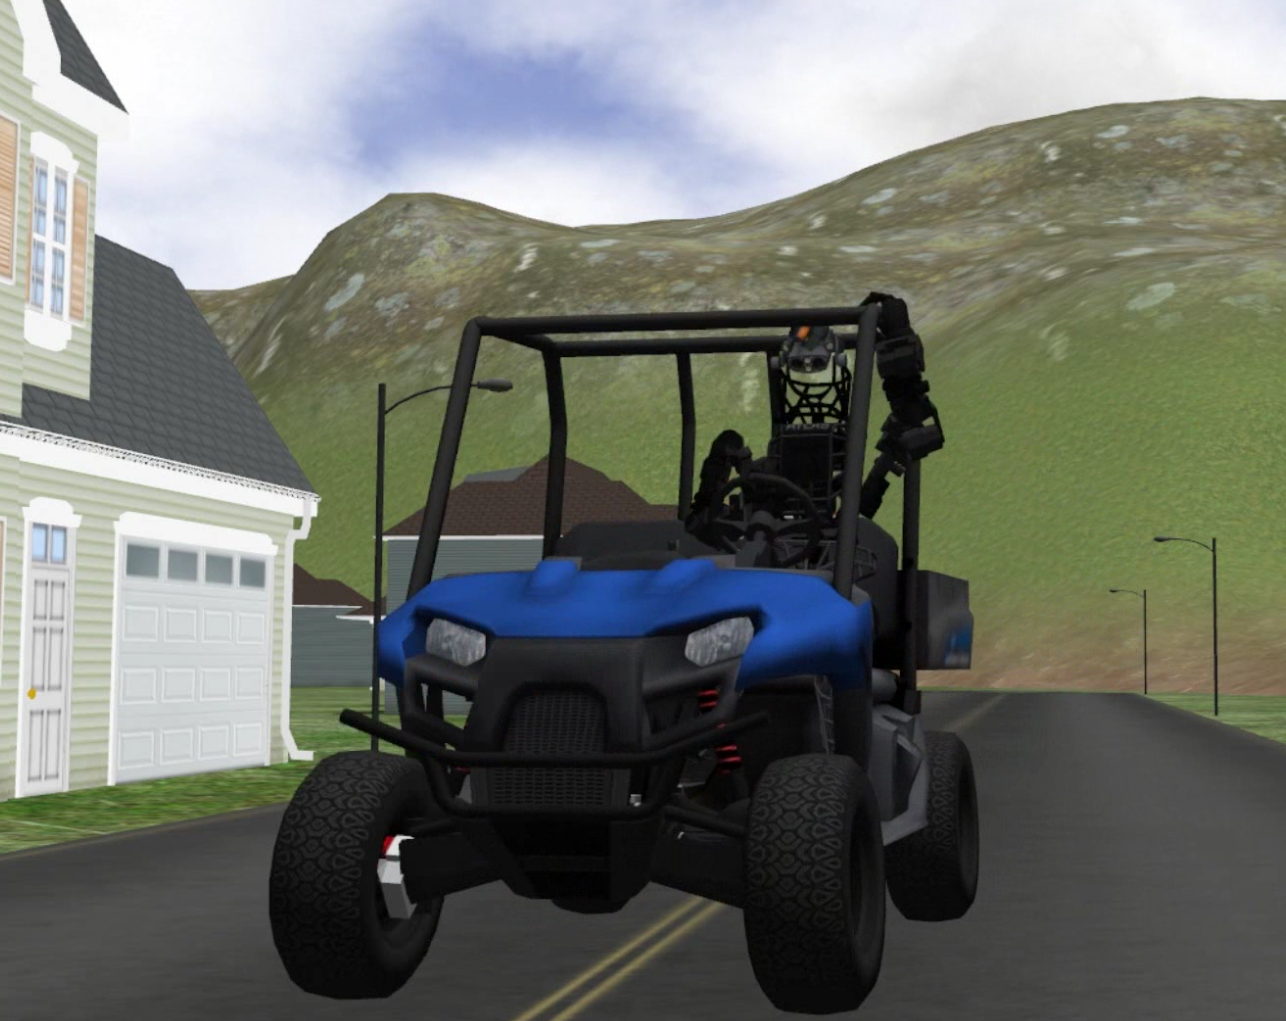
\includegraphics[width=\textwidth]{pics/darpa_car}
    \caption{Driving a car}
    \label{fig:vrc_car}
  \end{subfigure}
  \begin{subfigure}[b]{0.3\textwidth}
    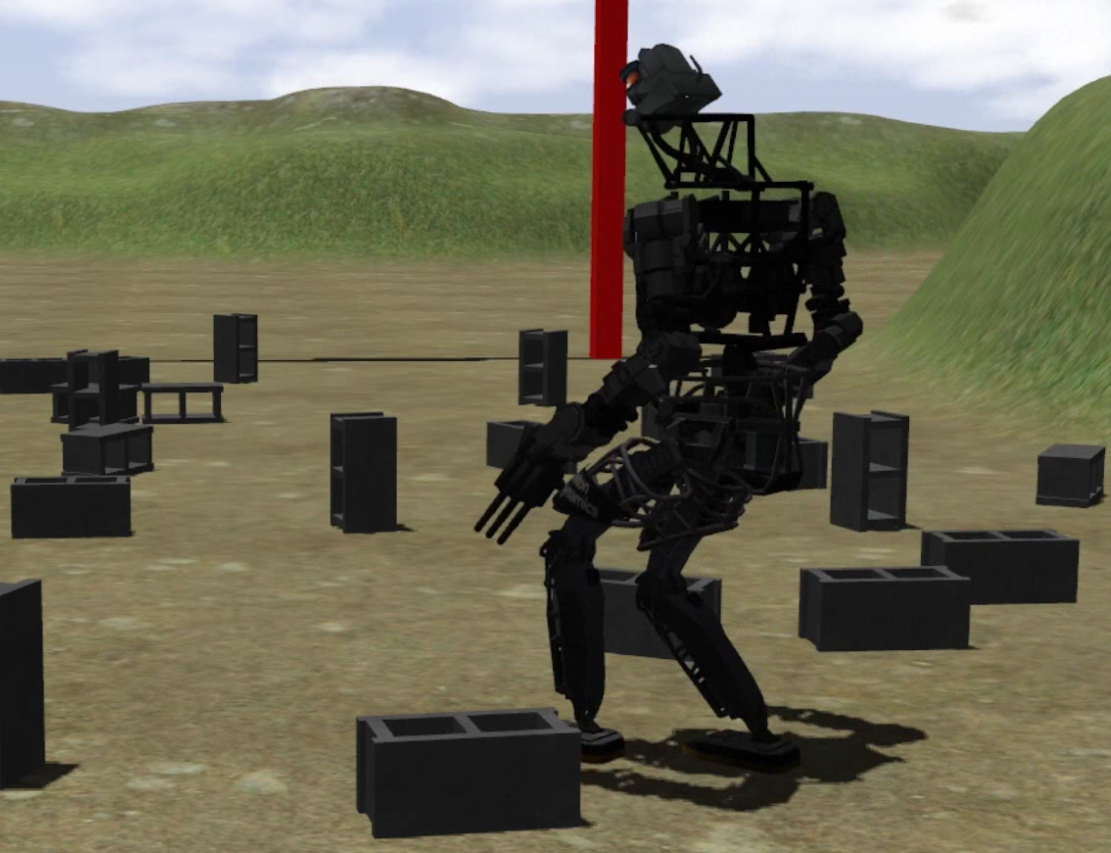
\includegraphics[width=\textwidth]{pics/darpa_walking}
    \caption{Crossing rough terrain}
    \label{fig:vrc_walking}
  \end{subfigure}
  \begin{subfigure}[b]{0.3\textwidth}
    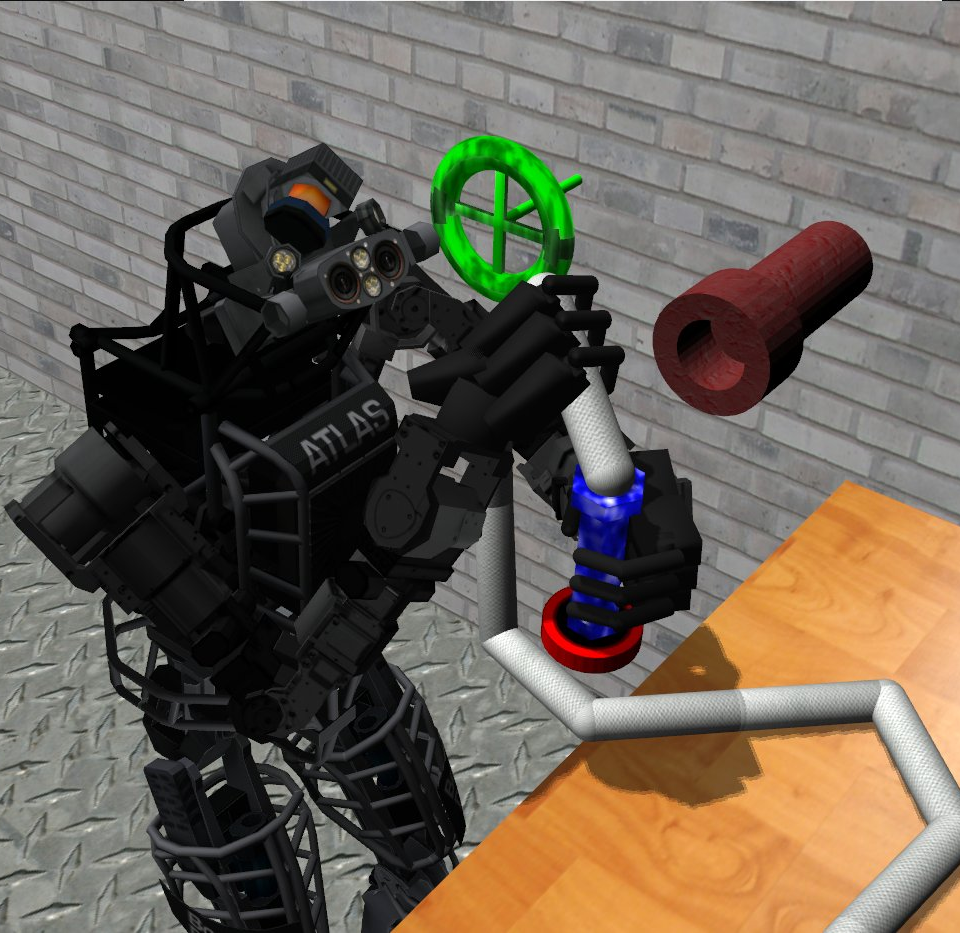
\includegraphics[width=\textwidth]{pics/darpa_hose}
    \caption{Connecting a hose}
    \label{fig:vrc_hose}
  \end{subfigure}
  \caption{Tasks of the Virtual Robotics Challenge~\cite{vrc_pics}}
  \label{fig:vrc}
\end{figure}
In the first task, the robot has to walk to a car, enter it and drive along a street. The chassis of the car consists of a framework to simplify the entry. On the road, there are obstacles the robot has to avoid. The second tasks tests the walking capabilities of the robot. The robot has to cross slippery and irregular terrain to test balancing and a terrain with obstacles to test perception and footstep planning. The last task is about manipulation. The robot has to connect a hose to a pipe by plugin it in and screwing it down. Afterwards, it has to open a valve. All tasks have randomized parameters, such as the position of obstacles and goals.\\
VRC is related to this thesis because it also uses the Gazebo simulator~\cite{IEEESpectrum}. Therefore it shows what Gazebo is capable of and how important a simulation is for the development and research of cutting-edge technology. \textcolor{red}{more}
Although the technology fostered by DRC is important and useful without doubt, it seems questionable what DARPA as a military agency will use this technology for.


\subsection{RoboCup Simulation Leagues}
In the RoboCup competition, there are different simulation leagues. On the one hand, there are the 2D and 3D soccer simulation leagues and on the other hand, there are two rescue simulation leagues. In all of those leagues, multi-robot coordination is a important field. This is not surprising because it is much simpler to benchmark multi-robot strategies in a simulation. There is no need to operate real hardware and difficult low level control and sense problems, that are not the focus of the benchmark, can be simplified or left out.\\
\begin{figure}
  \centering
  \begin{subfigure}[b]{0.48\textwidth}
    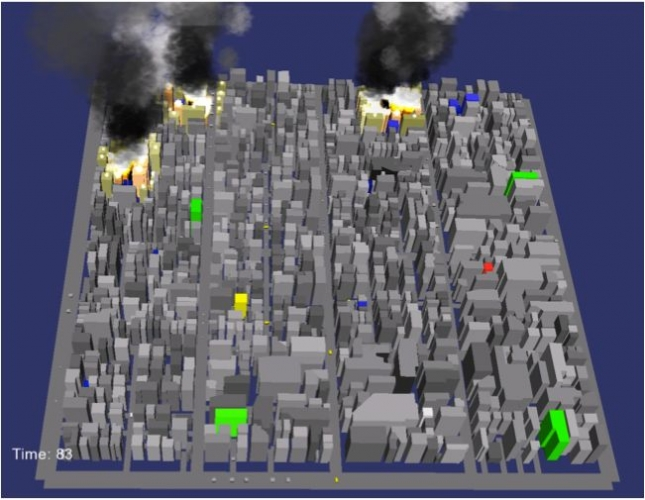
\includegraphics[width=\textwidth]{pics/rescue3d}
    \caption{Agent Competition~\cite{rescue3d}}
    \label{fig:rescue_agent_competition}
  \end{subfigure}
  \begin{subfigure}[b]{0.48\textwidth}
    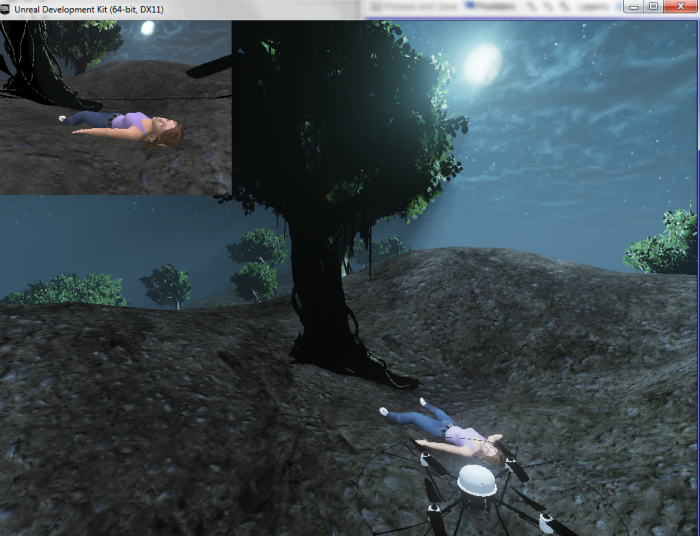
\includegraphics[width=\textwidth]{pics/rescue_vrc}
    \caption{Virtual Robot Competition~\cite{rescue_simulation_league}}
    \label{fig:rescue_vrc}
  \end{subfigure}
  \caption{Rescue Simulation Leagues}
  \label{fig:rescue}
\end{figure}
The \textit{Rescue Simulation League (RSL)} aims to benchmark intelligent software agents and robots in a disaster scenario~\cite{rescue_simulation_league}. RSL is separated into to leagues with different with focus on different scales. Figure~\ref{fig:rescue} shows snapshots of both simulation. The \textit{Agent Competition} is about a large scale disaster in a city with multiple robot teams. The \textit{Virtual Robot Competition} is about finding victims in a burning house or limited outdoor area with a team of eight robots and one human operator. The operator can give high level commands, such as the area where to look for victims, and is needed to verify the observations of the robots. So, the robots should find and approach victims autonomously and the operator has to confirm it. The task of the agents include victim-detection, autonomous generation of maps, navigation and multi-robot coordination. In the Agent Competition, there is no realistic robot control and perception necessary. The focus is on the coordination of many heterogeneous agents to take high level decisions. There are teams of fire brigade, police and ambulance, each with up to 30 simulated agents. Each agent acts autonomously and can communicate with other agents. The tasks of the agents include exploration, scheduling and planning in cooperation with other agents and building of agent teams (e.g. to fight fires more effectively).\\
\begin{figure}
  \centering
  \begin{subfigure}[b]{0.48\textwidth}
    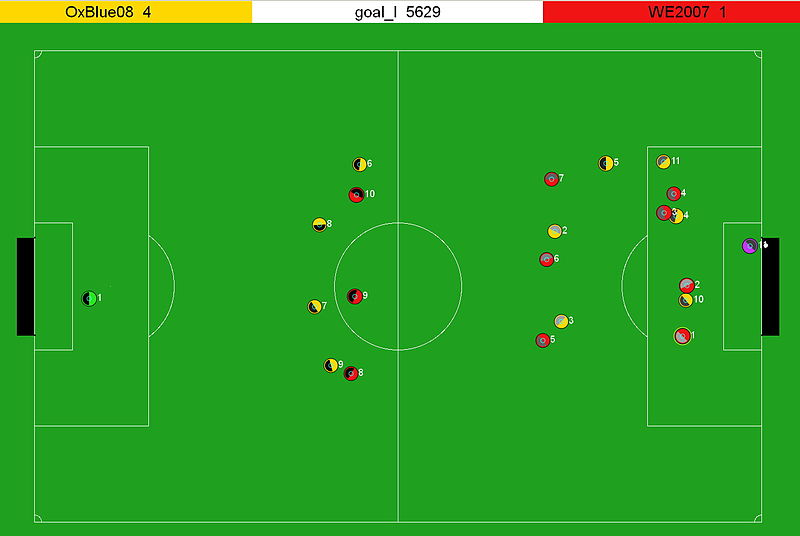
\includegraphics[width=\textwidth]{pics/soccer_simulation_2d}
    \caption{2D Soccer Simulation League~\cite{soccer_simulation_2d_pic}}
    \label{fig:soccer_simulation_2d}
  \end{subfigure}
  \begin{subfigure}[b]{0.48\textwidth}
    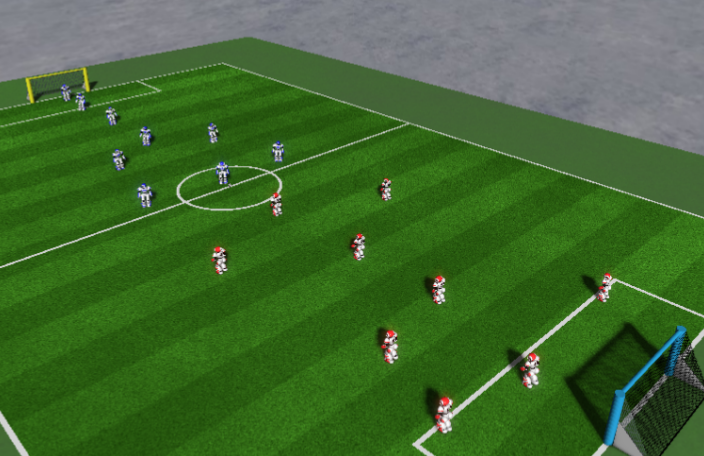
\includegraphics[width=\textwidth]{pics/soccer_simulation_3d}
    \caption{3D Soccer Simulation League~\cite{soccer_simulation_low_level}}
    \label{fig:soccer_simulation_3d}
  \end{subfigure}
  \caption{RoboCup Soccer Simulation Leagues}
  \label{fig:soccer_simulation}
\end{figure}
The soccer simulations of the RoboCup are similarly split in two leagues. In the \textit{2D Soccer Simulation League}, 22 agents in two teams play soccer in a two dimensional environment. A single server called Soccer Server simulates and controls the game with its physics, the actions of the agents and the perception of the agents. Each agent is an autonomous program and communicates with the soccer server to receive noisy sensor data and send action-commands to influence the simulation~\cite{soccer_simulation}. The main challenges of the 2D Soccer Simulation League are planning the actions of each agent when playing in offense and reacting on the opponent and predicting his movement when playing in defense. The \textit{3D Soccer Simulation League} features a more realistic simulation. This league fully simulates nine NAO robots per team. Therefore, the low level control and perception are an important part of the challenge~\cite{soccer_simulation_low_level}. This is an important opportunity for the teams participating in SSL to test their approaches first in the simulation because SSL also uses the NAO as robot platform. The communication between the agents and the Soccer Server is in this league similar to the 2D league. The rules of the league are inspired by the FIFA football rules but have some reasonable extensions~\cite{soccer_rules_3d}. For example a goal directly form the kick off is not allowed and if too many robots are in a small area around the ball, the position of some robots is reset.\\
All simulations we have looked at in this section are similar to the simulation we developed for LLSF. The simulations are important for benchmarking multi-agent systems because the system can be tested with low effort in comparison with real multi-robot systems and some details, such as low level control and perception, can be left out.  Furthermore the simulations have in common that the evaluation of the whole system can be done by looking at the results and progress of the simulated games. Especially by 2D Soccer Simulation teams, this is used by to do reinforcement learning~\cite{simsoccer_reinforcement_1,simsoccer_reinforcement_2}. Similar as it is possible to improve a real multi-robot system in SPL by improving the performance of the multi-robot system in the 3D Soccer Simulation League~\cite{from_sim_to_real}, we also want to improve our real system by using a simulation.\textcolor{red}{ausfuehren?}


\subsection{Scene Reconstruction for Fault Analysis}
Some work was already done with Gazebo and Fawkes. Bastian Klingen developed a scene reconstruction for fault analysis in his diploma thesis~\cite{KlingenDA}. The scene reconstruction was primarily made for a mobile robot with a \textcolor{red}{Microsoft} Kinect and a laser range sensor for perception and a gripper arm for manipulation. The task of the robot was to grep a colored cup on a table. The scenario and the reconstruction are shown in Figure~\ref{fig:klingen}. Because this gripping task involves many components and sometimes fails if a single component fails, a tool was needed to analyze unsuccessful attempts afterwards. This tool reconstructs the scene with the position of the robot, its sensor data and world belief. Therefore the movements, sensor data and belief of the robot have to be logged while performing a grep. The logging was also done with MongoDB because of the needed speed. Gazebo was used to visualize the robots perception and belief and to reconstruct the scene. Fawkes was used to control the robot, to log the needed data and to control gazebo and read the log while reconstructing the scene. Together with the scene reconstruction, Klingen provided a tool to analyze faults to find components that causes the faults. Therefore he constructed a dependency tree of the components and ordered it in a data-information-knowledge hierarchy.\\
\begin{figure}
  \centering
  \begin{subfigure}[b]{0.38\textwidth}
    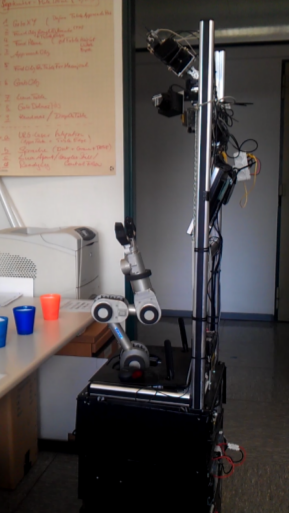
\includegraphics[width=0.7\textwidth]{pics/klingen_real}
    \caption{Grasping a cup in the real scene}
    \label{fig:klingen_real}
  \end{subfigure}
  \begin{subfigure}[b]{0.58\textwidth}
    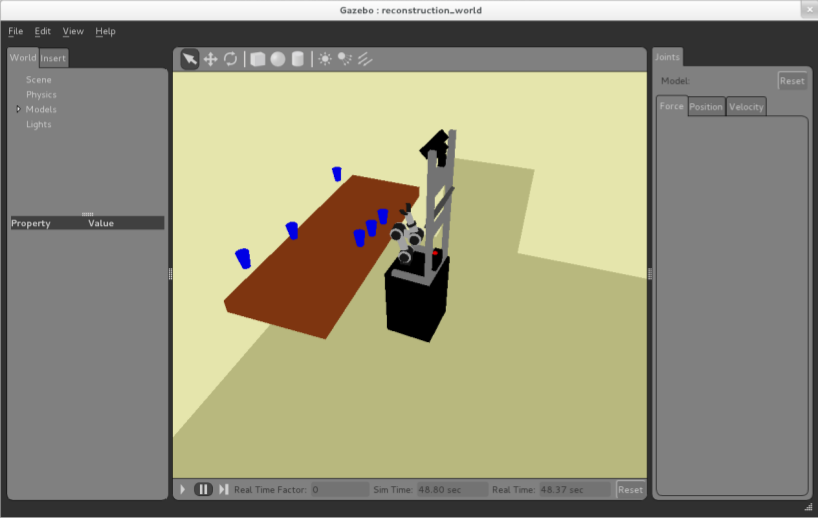
\includegraphics[width=\textwidth]{pics/klingen_sim}
    \caption{Reconstruction in the Gazebo simulator}
    \label{fig:klingen_sim}
  \end{subfigure}
  \caption{Scene Reconstruction for Fault Analysis~\cite{KlingenDA}}
  \label{fig:klingen}
\end{figure}
To establish the communication between Fawkes and Gazebo, Klingen developed a Fawkes plugin that provides the communication objects of the Gazebo \textcolor{red}{API} as an aspect. In this thesis we use this plugin and expend it for our needs. Similar but not so sophisticated as in the thesis by Klingen, we want to provide a possibility to reconstruct faults to find the causes. We do not record the perception of the robots in the simulation but we record the movement of all simulated objects and the high level decisions of the agents which represent can be used to derive the belief of the robot. The motion of the objects in the simulation can be recorded by Gazebo and the agent decisions by logging our rule-based production system CLIPS. We describe CLIPS in \textcolor{red}{a following section or the background}.

\subsection{Simulation Environment for the Middle Size League}
An other work with Gazebo and Fawkes developed a simulation environment for MSL~\cite{MultiLevelAbstraction}. This simulation environment became necessary because the field size and the amount of robots per team was increased in MSL. Therefore testing became more difficult. The work used an early version of Gazebo and Player as interface between Fawkes and Gazebo. On the one hand, it showed that the Gazebo simulator is capable of complex components of the robot that cause problems in other simulators. This was shown for omni-directional wheels an an omni-directional camera. \textcolor{red}{Omni-directional wheels can move in one direction similar to normal wheels and have small rolls at the outside of the wheel to be able to move in an other direction without resistance. An omni-directional camera consists of a upwards faced camera and a hyperbolic mirror above, so that the camera can see the whole area around the robot.} Both devices are non-trivial to simulate and often used in MSL. The Robotino we use in this thesis also holds these two devices. On the other hand, the work proposed the idea of \textit{multi-level abstraction}. If a robot software contains separate components for steps that are based on each other, it is useful to simulate not only the hardware level, the lowest abstraction level, but also higher abstraction levels. For example if the robot software includes a component that reads an image from a web-cam and a component that computes the state of a traffic light from this image, the simulation can provide the simulated image as well as the information about the traffic light. A simulation with multi-level abstraction is able to switch between different abstraction levels. This can be useful to test components on a higher level independent of low level components which can introduce an error or are not finished. Multi-level abstraction has the additional advantage that the components of a higher abstraction level often can be simulated with less computational effort. This makes it easier to run the simulation on a slow computer. However it is not always reasonable to introduce multiple abstraction layers, because some components, such as a collision avoidance, can not be simulated easily. In this thesis, we also use multi-layer abstraction to be able to test high level components more individually.


\section{Multi-Agent Strategies}
\label{sec:multi_agent_strategies}
In this section, we present our current high level agent approach, which we want to evaluate and improve during the thesis. We also present some advanced and attractive multi-agent strategies. On the one hand our simulation should be able to simulate and evaluate these approaches as well and we might want to use one of these approaches because our current one has some limitations.

\subsection{Incremental Task-level Reasoning}
Our current implementation of the high-level agent uses the CLIPS rules engine. Our implementation is based on the idea of incremental task-level reasoning~\cite{Incremental}. This means that the agent takes the next best possible action whenever the robot is idle. Simplified, every action is represented by a CLIPS rule. The action is possible if the antecedent of the rule can be matched by the fact base. The consequent of the rule include the execution of the action itself and changes to the fact base to remember the current situation. If new perception data is available for the agent or the execution of an action finished or failed, this is asserted as a fact and can therefore cause in the application of some rules to update the belief of the agent in the fact base or to execute the next best action. If more than one action is possible, the action with the highest priority is executed. \textcolor{red}{example?}\\
The incremental reasoning approach with CLIPS has several advantages. Actions and handling perception can easily be represented by rules which work with the current belief of the agent, the approach is computationally inexpensive, because no costly planning is needed, and it is easy to cope with incomplete knowledge because the agent just takes the next best action and updated its belief if new information is available. \textcolor{red}{2012 kuerzen?} In the LLSF competition of 2012 incomplete knowledge was a part of the problem because the robots had to find out the types of the machines by trying how they react on different input pucks. The refbox, which was introduced in 2013, now provides the information about the machine types. However, dealing with incomplete knowledge is still important, especially if the agent recognizes that it made a mistake and the world belief is partially wrong.\\
To coordinate the agents working simultaneously, until the RoboCup 2013 we have been using only two robots, we use a role based approach with additional resource locking. Every agent has a specific role, which determines for which tasks the agent is responsible for and which machines it can use. We have one role for an agent which only produces P3 pucks and delivers them. This agent continuously provides easy points because P3 is the simplest product, that needs only one resource puck (see Figure \ref{fig:llsf_chain}). In the following, we call this role the \textit{P3-role}. A second role is responsible for producing  more complex products, the P1 and P2 pucks. This role can provide a large amount of points but is more risky because of the higher amount of intermediate steps. We call this role the \textit{P1P2-role}. Whether the P1P2-role produces P1 or P2 pucks is determined by the distance between the needed machines to the machine for P3 products. This spacing is necessary because the different robots drive independently and it can take a while if the have to pass each other when their paths cross. Most of the objects in LLSF, such as machines and the delivery zone, can only be used by one robot at a time. Therefore we implemented a master-slave resource locking mechanism for the agents. If an agent decided to drive to a position, he requests the lock of this position and waits till he receives the lock. Then he drives there and frees the lock when he leaves the position. The roles are also used for multi-robot coordination in the exploration phase. The roles determine which machine an agent investigates first. After the first machine, the agents continue the investigation of the other machines in the same cycle till all machine types are identified. The agents can pass each other on the cycle.\\
It is easy to see that the current approach has limitations which obstruct a significantly better performance. The static roles do not allow a tight cooperation between the agents. For example, a tighter cooperation would allow us to produce P1 and P2 pucks faster because the agents could split the work. AN other problem of the static roles are that the agent behavior often can not take the situation into account. For example if there is not enough time to produce an other P1 or P2 puck or there are no more P1 or P2 pucks ordered, the P1P2 role would still start start another production.\\
There already is a less sophisticated simulation, which is able to test if the high-level-agent basically works. This simulation is implemented within the CLIPS-agent and provides information about the execution of actions and perception results in a trivial way. A few seconds after every action called from the agent, the action is reported as successful and the perception results match exactly the ground truth published by the refbox. This is useful to test the behavior of the agent in the best-case scenario. Though, this simulation is only able to simulate the actions of the agent and can therefore not indicate many important real world problems. Furthermore the simulated situation is not graphically visualized and therefore difficult to evaluate. Testing and evaluate multi-robot coordination is also not possible in this simulation because every agent uses an own simulation and the different time-spans for different actions can not be taken into account.

\subsection{Marked Based Strategies}
\textcolor{red}{more task allocation strategies with e.g. dynamic role assignment?}\\

The simulation should be able to test and compare complex multi-robot coordination strategies. An example of such a strategy, which is attractive for our needs and used for orientation in the design process of the thesis, is \textit{Murdoch}~\cite{DissMurdoch}. Murdoch is an auction-based task allocation strategy. It solves a special instance of the \textit{Optimal Assignment Problem}. The Optimal Assignment Problem is to assign $n$ weighted jobs to $m$ workers with non-negative skill ratings $h_{i,j}$ for each worker-job combination. Each worker is capable of doing one job at a time and each job can only be done by one worker. The task is to find the assignment which optimizes the performance, taking into account the weights of the jobs and the skill ratings of the workers to the jobs. The Murdoch method was especially developed 
for multi-robot scenarios. Therefore, it was designed to be able to handle robot failure and communication message loss. If a robot discovers a new task, it becomes an auctioneer and publishes a broadcast message to inform other robots about the task. All robots that are capable of doing the task calculate a metric of how well they probably will perform on the task. The metric is sent as a bid to the auctioneer. Finally, the auctioneer decides after a predefined time interval which robot gets the task and informs this robot. After the allocation, the auctioneer observes the progress of the task and starts a new auction if the robot assigned in the first place fails. This method is to some degree decentralized because the different auctions and metric calculation are not executed by a single robot. However, this approach is not optimal for a set of tasks because every auction only considers a single task. \cite{DissMurdoch}~showed that the method performs well in different multi-agent tasks, such as cooperative manipulation.\\
Murdoch allows a dynamic and situation dependent task allocation and is especially well suited for heterogeneous robots with different abilities. It is also a useful method to allow reallocation of tasks. An agent which is executing a tasks and has already completed a part could change his task if a new task is more important. The agent could simply include the penalty, that it has to cancel a task, and the advantage, that it has from completing the previous task, in his bid for the new task. An example in our domain is a robot which is carrying an intermediate product S1 for the production of a new P1. If a S1 is needed at an other machine with higher importance, the robot can change the task. The cancel of the old task is no problem because the agent can just start a new auction for the old task. Disadvantages of Murdoch are the high demand of communication and the difficulty to detect failures.

\chapter{Approach}
\label{cha:approach}
In this chapter, we describe the approach of this thesis by presenting the main ideas to reach our goals for the simulation and high-level agent in section~\ref{sec:goals_and_approaches}. In section~\ref{sec:architecture}, we present the architectural approach.

\section{Goals and Approaches}
\label{sec:goals_and_approaches}
\textbf{Realistic simulation:} An important goal of the thesis is a high realism of the simulation. The realism can be defined by the similarity of sensor data and consequences of robot actions between simulation and reality. A more realistic simulation allows more compete testing because more real problems can be simulated. The realism of the simulation has many different aspects. The first group of aspects is about the realism of sensor data. There are some sensors that are easy to simulate, such as distance sensors, bumpers and gyroscopes. Others, especially cameras, are more difficult to simulate realistically. The choice of Gazebo with ODE and Ogre for the visual appearance already allows us to simulate a wide range of sensors realistically. Also the noise in the sensor data is important for the realism of the simulation. For all metric sensors, we simulate this as Gaussian noise with the calculated value as mean and a configurable variance. The second group of aspects are about the realism of the physical environment. Objects have to behave in the simulation and the reality in a similar way. This is especially important for robot movement and manipulation tasks. Here, Gazebo with ODE also provides high realism out of the box. Nevertheless, it is important to find good physical parameters for the simulated objects. Examples of those parameters are the mass and coefficients of friction. Another important aspect of simulation-realism is that the simulation should not introduce new problems which do not occur in reality. Such a problem, which occurred in the development of the thesis, is that the simulation ran slower than the system time but the robot software used the system time. This caused to early triggering of timeouts. We solve this problem by providing the simulation time in Fawkes.\\
\textbf{Different levels of simulation:} Sometimes, it is also useful to test with a more abstract and less realistic simulation. This allows testing the optimal case without sensor noise or without using low level components, such as localization, if those produce new errors or are not finished yet. To be able to simulate on different levels, we use the multi-level abstraction approach~\cite{MultiLevelAbstraction} presented in the chapter~\ref{cha:related_work}. We use multi-level abstraction for sensing and for actuators. How we use multiple abstraction levels is shown in the next section about the architecture.\\
\textbf{Compatibility with original robot software:} We want to achieve that the robot software runs in the same way in the simulation as in reality. This is important because otherwise it would result in additional effort to keep the robot software running in the simulation. This effort can also cause more difference between simulation and reality. In the thesis, the simulation components should provide the same interfaces as the real components that are simulated. In Fawkes, this is easy to achieve because the interfaces between components are well defined and components using an interface do not recognize whether the interface is provided by the simulation or a real component.\\
\textbf{Efficient testing:} We want to make the use of the simulation as efficient as possible. To achieve this, we provide scripts which automatically start the full simulation with all needed programs. Without these scripts, it would take much more time. For a full simulation of an LLSF game, it is necessary to start Gazebo, the Refbox, a controlling Fawkes instance and, for the Robotinos, three times Fawkes, \texttt{roscore} and \texttt{move\_base}. Each program-instance has to be started with correct parameters.  Another approach we use to increase the efficiency is the feature to load different configurations and setups. For example, the scripts are able to load the simulation with different numbers of Robotinos, abstraction levels and simulation environments. Loading different configurations for the robot software is a feature of Fawkes and useful for us. We also integrated this into the scripts. Furthermore, we provide the possibility to draw objects into the simulation. This makes it possible to visualize belief and intention of a robot to identify mistakes or ways to improve the system~\cite{Visualization}.\\
\textbf{Multi-robot system evaluation:} An important part of this thesis is the evaluation of multi-robot systems. Here, the features we already mentioned in the previous paragraph are especially useful because the testing effort (e.g. to setup the simulation or analyzing the coordination between robots) often scales with the number of robots. To evaluate the performance of the multi-robot system faster without having to observe the simulation all the time, we provide the possibility to run multiple simulation runs, in our case runs of LLSF games, automatically. With this feature, the simulation can run, for example, 20 times over night. To analyze executed simulation runs, we keep statistics of each run. For our LLSF domain, we keep the amount of achieved points with a detailed list of all actions that provided points with the time. These statistics can easily be extended by the amount of collisions between robots, waiting time for resource locks or other useful measurements. Sometimes, it can happen that single simulation runs have a very different results. To find the reason for this result, we keep log files of each run and also record the simulation itself. With this record, the simulation run can be reconstructed. The record contains the position and movements of all objects in the simulation. Here, it is also useful to draw additional information, such as the localization of the robots, in the simulation to be able to analyze faults without having to look in the log files. Automated simulation runs also allow the comparison of different configurations of the multi-robot system. The automation script can be started with a number of configurations to test. This can be useful for finding the best performing role combination or parameters such as thresholds.\\
\textbf{Expandability and flexibility:} An essential criterion of a good simulation is the expandability to adapt to future changes. On the one hand, there will be changes to the Carologistics Robotino and to the LLSF. These changes have to be easy to implement in the simulation, otherwise the simulation would not remain useful. On the other hand, it is attractive to use the simulation also in other domains, such as RoboCup@Home. To achieve the expandability of the simulation, we provide a framework for simulated devices in Gazebo and Fawkes. Furthermore, we focus on developing small modules that are exchangeable and reusable. In Gazebo, new modules can easily be added to robot and world plugins. In Fawkes, it is easy to implement a new plugin which provides the wanted features because the plugin can use the provided Gazebo aspect. The simulation should also be flexible to adapt to small changes. Therefore, we provide several configuration files for the simulation environment, for the simulated objects and robots and for plugins in Gazebo and Fawkes.\\
\textbf{Agent improvements:} It is easy to see that the current approach we showed in section~\ref{sec:multi_agent_strategies} has limitations which obstruct a significantly better performance of our multi-robot system. The static role approach does neither allow a tighter cooperation between the agents nor that the agent behavior can take the situation into account. For example, if there is not enough time to produce another $P_1$ or $P_2$ puck or there are no more $P_1$ or $P_2$ pucks ordered, the $P_1P_2$ role would still start another production. Therefore, we want to introduce a dynamic role change to switch roles in specified situations. Furthermore, we want to introduce recycling because it can lead to simple points and provides an alternative possibility to get new $S_0$ pucks. A third way to improve the performance of our system is to make use of three robots instead of just two.\\


\section{Architecture}
\label{sec:architecture}

\subsection{Simulation}
\label{sec:architecture_simulation}
\begin{figure}
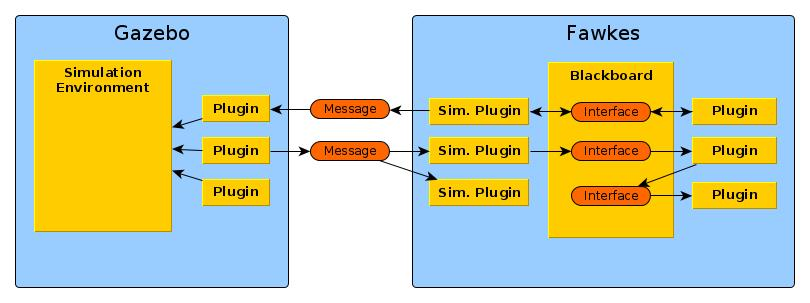
\includegraphics[width=\textwidth]{tabs/fawkes_gazebo}
\caption{Architecture of the simulation}
\label{fig:fawkes_gazebo}
\end{figure}
The basic structure of the simulation is shown in Figure~\ref{fig:fawkes_gazebo}. On the right side, there is the Fawkes robot software framework we want to run in the simulation. On the left side, there is the simulator Gazebo. Roughly, the simulation is composed of a simulation environment, which handles the physical and visual simulation of the environment with all included objects, and plugins associated to the world and all models with some kind of behavior. There are plugin instances for the sensors and actuators of each robot as well as plugins that control the world. At this point, Fawkes can be seen as a composition of plugins, which are used on the real robot system, simulation plugins, which communicate with the simulation and exchange original sensor and actuator plugins, and the blackboard. The blackboard manages several interfaces which are used for communication between Fawkes plugins. The Fawkes simulation-plugins send actuator messages to the corresponding Gazebo plugins and receive messages from sensor-plugins in Gazebo. This architecture has the advantage that it is flexible and extendable. To add a new sensor or actuator to the simulation, it is sufficient to create or modify a Gazebo plugin and a Fawkes simulation-plugin to provide the corresponding interface. Furthermore, the architecture is flexible enough to allow multi-level abstraction as we see later in this section. It is also easy to change plugins on either side. It is even possible to use the Gazebo simulation with another robot operating system than Fawkes. The other system just has to send and receive the same messages as our simulation-plugins.


\subsection{Communication Fawkes-Gazebo}
\label{sec:architecture_communication}
\begin{figure}
\center
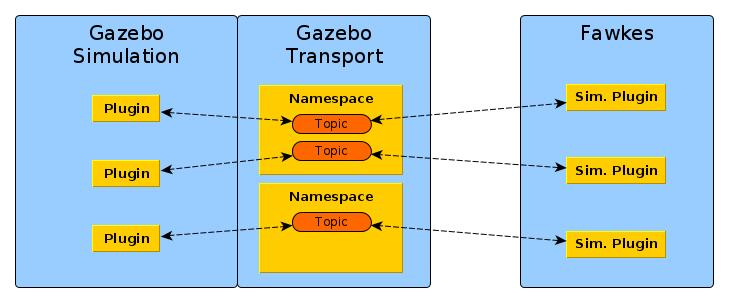
\includegraphics[width=\textwidth]{tabs/communication}
\caption{Communication between Fawkes and Gazebo}
\label{fig:communication}
\end{figure}
The communication between Fawkes and the Gazebo simulation has a specific structure to organize the distinction between multiple robots and different sensors and actuators. Figure~\ref{fig:communication} shows this structure. Fawkes simulation-plugins and Gazebo plugins communicate over a message-transport system. In our case, this system is embedded in the Gazebo Transport API. In the message-transport system, there are different namespaces which act as communication channels. There is one namespace for each simulated robot and for the simulated world. The topics in a namespace represent what the messages that are sent on this topic are about. Each plugin can listen to or send on the topics in a namespace. For example, there are topics about laser data and motor commands. This architecture is extendable because it is easy to add new namespaces or topics. It is flexible, because the communication through a topic in a namespace is a many-to-many relationship, and it is comfortable because instances of plugins in different Fawkes instances can listen to the same topic and get data from different simulated robots because the plugins listen do different channels.


\subsection{Multi-level Abstraction}
\label{sec:architecture_mla}
\begin{figure}
\centering
\begin{subfigure}[b]{\textwidth}
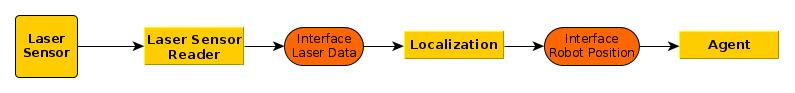
\includegraphics[width=\textwidth]{tabs/mla_hardware}
\caption{With real hardware}
\label{fig:mla_hardware}
\end{subfigure}
\begin{subfigure}[b]{\textwidth}
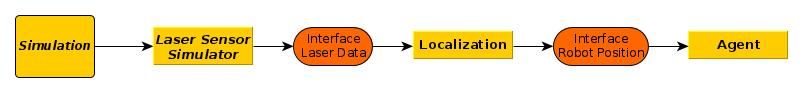
\includegraphics[width=\textwidth]{tabs/mla_sim_low}
\caption{With low level abstraction}
\label{fig:mla_sim_low}
\end{subfigure}
\begin{subfigure}[b]{\textwidth}
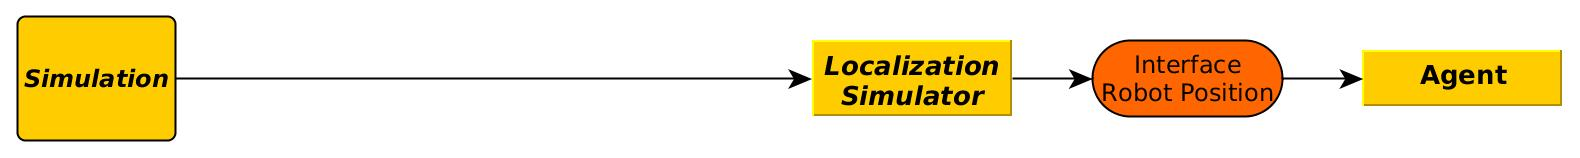
\includegraphics[width=\textwidth]{tabs/mla_sim_high}
\caption{With high level abstraction}
\label{fig:mla_sim_high}
\end{subfigure}
\caption{Example for multi-level abstraction (The arrows indicate data flow.)}
\label{fig:mla}
\end{figure}
Figure~\ref{fig:mla} shows how multi-level abstraction fits into our simulation architecture. We choose a simple example about the localization with laser data. Figure~\ref{fig:mla_hardware} shows the system as it is used in the real application. There is the laser sensor hardware, a plugin which reads out the sensor and publishes the laser data in an blackboard-interface, a localization plugin which uses the laser data interface to determine a robot position and to provide the position in another interface. Then, the robot agent uses the position information from the interface. Figure~\ref{fig:mla_sim_low} shows the system in the simulation with low level abstraction. The hardware is replaced by the simulation and the laser sensor reader by a simulation-plugin which receives the laser data from the simulation. This simulation-plugin provides the same interface as the original plugin. Another possibility with high level abstraction is shown in Figure~\ref{fig:mla_sim_high}. Here, the localization plugin is replaced by a simulation-plugin which simply looks up the position of the robot in the simulation and writes it in the interface. The agent can now be simulated with ground-truth position data without using of the original localization plugin. An example for multi-level abstraction for actuators could be the movement of a robot. It is possible to simulate the motors with motor commands from an interface or the motion of the robot by applying the motion command in an interface directly to the simulated robot.

\chapter{Implementation}
\label{cha:implementation}
In this chapter, we describe how we implemented the simulation. First, section~\ref{sec:components} presents the various components we developed by describing what their task is, what we noticed during the implementation and why we implemented it this way. \textcolor{red}{module dependencies extra or in modules?} In section~\ref{sec:module_dependencies}, we describe the dependencies and interaction between the modules we developed. Section~\ref{sec:imp_communication} covers the implementation of the communication between Fawkes and Gazebo and between multiple robots we want to simulate. In section~\ref{sec:agent_improvements}, we present the improvements for the multi-agent system we implemented during the thesis.

\section{Components}
\label{sec:components}
\subsection{Gazebo Models}
\begin{figure}
\centering
\begin{subfigure}[b]{0.48\textwidth}
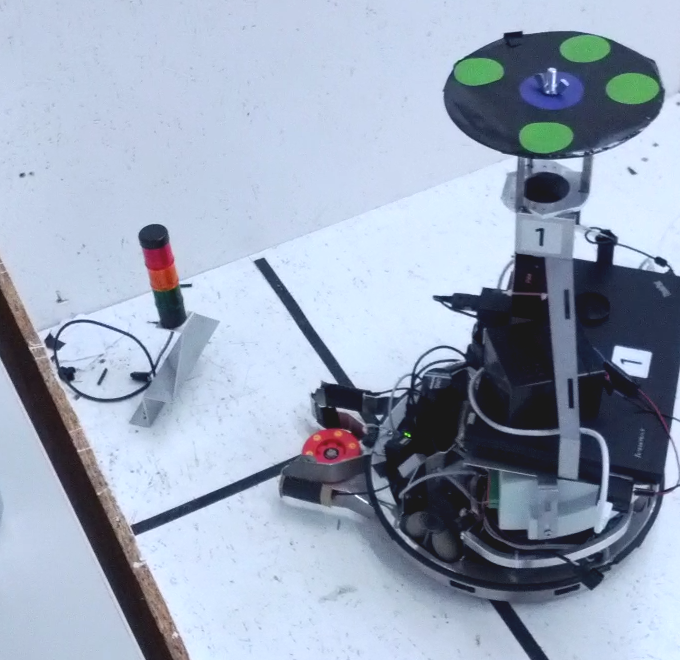
\includegraphics[width=\textwidth]{pics/llsf_real}
\caption{A Robotino delivers a puck to a recycling machine.}
\label{fig:comparison_real}
\end{subfigure}
\begin{subfigure}[b]{0.48\textwidth}
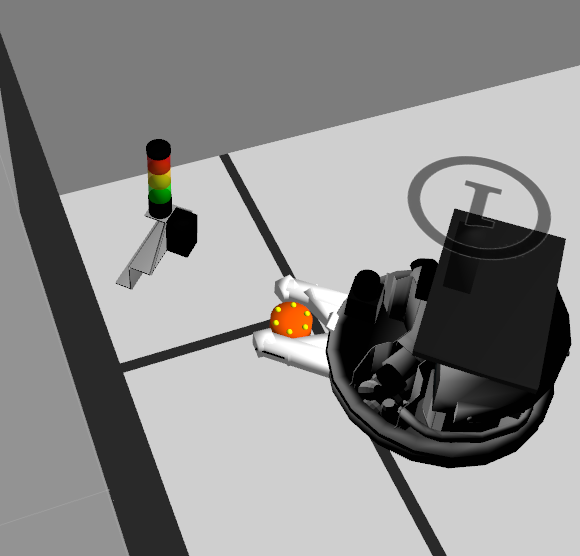
\includegraphics[width=\textwidth]{pics/llsf_sim}
\caption{The same situation in the Gazebo~simulation}
\label{fig:comparison_sim}
\end{subfigure}
\caption{Comparison of the real scene and the simulated scene in Gazebo}
\label{fig:comparison}
\end{figure}

In order to simulate the LLSF environment, we need to model all objects appearing in this domain. The models developed in this thesis are available at \url{https://github.com/zwilling/llsf-models.git}. Here, we present our simulation models and why we modeled them this way. Figure~\ref{fig:comparison} shows a comparison between a real LLSF scene and the same scene in the simulation. In this comparison, the most important objects of the simulation can be seen. In the following, we describe each model in detail:\\
\textbf{LLSF Field:} The model of the LLSF field has a rather simple structure. It consists of a ground plate and four side walls. For the visual appearance and possible future changes, the field has a visual representation with lines and colored areas just as on the real field. The machines are not realized as a component of the field and are attached to the field in the description of the simulation world.\\
\textbf{Machine:} The model of the machines matches the real machines structurally. Though, it is challenging to represent the lamps consisting of colored Plexiglas and a LED \textcolor{red}{abbreviation?} inside. We decided to use simple colored cylinders in the simulation. If the lamp is turned off, we use a dark and slightly transparent color and, if the light is turned on, we use a a bright color. This looks reasonable in the simulation and the images from the simulation are sufficient for our vision plugin which determines the lamp state of the machines. The vision plugin measures the brightness at the position where it expects the machine-lamp to be and it even was not necessary to change brightness thresholds. In Figure~\ref{fig:comparison_real}, the black RFID box in front of the machine is missing because we currently do not have the RFID readers.\\
\textbf{Puck:} The visual appearance of the puck model can be seen in Figure~\ref{fig:comparison_sim}. Physically, they are represented by a single cylinder. The difficult part was to find good friction parameters for the surface of the cylinder. On the one hand, it should be easy to slide the puck across the floor. On the other hand, the puck should stay inside the gripper of the Robotino when the Robotino turns. If the friction parameters are too small, the pucks move outside the gripper while turning because of the centrifugal force. \textcolor{red}{mention other solution?}\\
\textbf{Robotino:} The model of the Robotino is the most complex model because it holds different sensors, the casing and the puck gripper. It is also the most important one because it represents the robot we want to simulate. The major visual difference between real world and simulation is caused by the missing framework on top of the Robotino and the visual appearance of the puck gripper. Both is not important because we do net detect other Robotinos with a camera. We detect them with the laser sensor. Therefore and because of the manipulation with the gripper, the physical representation is more important. \textcolor{red}{collisions picture?} The physical model of the Robotino is composed of the gripper and two cylinders, one on the ground to represent the basic circle of the Robotino and one on laser and machine height. The cylinder on laser height is smaller and shifted back so that it does not block the laser sensor of the same Robotino and it fits better to the real shape. The gripper in the simulation has a similar shape than the real one. We needed to assign higher friction parameters to the inside of the gripper than to the outside because in reality the puck slides into the gripper if the front side of the gripper and stays in the gripper while turning. Because we were not able to simulate this with a single set of friction parameters, we modeled an additional geometry for the inside of the gripper with higher friction parameters. Originally, we intended to add wheels to the physical design for the final version. However, the omni-directional wheels caused an abnormal physical behavior in the simulation. The wheels irregularly bounced on the ground because of gravity and collision. Because we could not solve this problem in an arguable time and there is no important advantage, we decided to stay at the simple model without wheels. We only loose the possibility to physically simulate the odometry with its error. Therefore we introduced an artificially odometry error in the Gazebo plugin for the Robotino. \textcolor{red}{friction, setvel?}\\
\textbf{Simulation World:} The world file combines the developed models to an LLSF environment. Our world consists of the LLSF field, 16 machines with configurable orientation, 20 pucks and three Robotinos.\\


\subsection{Gazebo Plugins}
plugins for robot and worlds consisting of smaller reusable modules \textcolor{red}{refactoring necessary}
\textbf{World Plugin}
\\
\textbf{Robotino Plugin}
\\
\textbf{Native Plugins}


\subsection{Fawkes Plugins}
The Fawkes plugins developed in this thesis provide access to the simulation in Fawkes. In order to identify plugins for the Gazebo simulation quickly, we named them with the prefix \textit{Gazsim}. We divided the plugins into two groups. The first group of plugins generally cover the access to the Gazebo simulation, sensors and the Robotino robot without limitation to a specific domain or task. All these plugins can be found in the simulation branch of the Fawkes repository\footnote{http://git.fawkesrobotics.org/fawkes.git}. The second group of plugins are needed for the simulation of the LLSF environment. They can be found in our LLSF repository\footnote{http://git.fawkesrobotics.org/fawkes-robotino.git} which includes the general Fawkes repository. The access to the LLSF repository currently is limited because it contains new code we want to take advantage of in the LLSF competition.

\subsubsection{Common Gazebo and Robotino Plugins}
\textbf{Gazebo:} The plugin called \textit{Gazebo} provides general access to the Gazebo Transport API which is needed to communicate with the simulator. Therefore, it provides a Fawkes aspect also called \textit{Gazebo}. After connection to the Gazebo simulator, the aspect gives access to two communication nodes. One node is responsible for the communication with the simulated robot Fawkes should control and has to be initialized with the name of the robot in the simulation. The other node is responsible for the communication with the simulation world and therefore used for robot independent information environment information. It is also possible to spawn new models and visuals through this node. This is useful for controlling of the simulation and visualizing tasks to show, for example, the robot intention. \textcolor{red}{bei klingen noch nicht multi-roboter faehig?}
\\
\textbf{Gazsim-Robotino:}
The \textit{Gazsim-Robotino} plugin exchanges the Robotino plugin which connects Fawkes with the hardware of the Robotino robot. Therefore our plugin provides the same interfaces as the original plugin. The original plugin provides motor and sensor features, each with an own interface. Because both are combined in the original plugin, we also combine these two features in the simulation plugin. However, we developed separate modules for these two features to improve re-usability. The module responsible for the motor sends the wished motor movement to Gazebo and receives the position of the robot in the simulation to compute the odometry. Because sending many Protobuf messages has been found to be computationally costly, we only send messages if he wished movement has changed. Here we also introduced an error to the odometry which occurs more strong when the speed changes quickly. As in reality, the odometry also changes if the robot drives against an obstacle and does not change it's position. \textcolor{red}{important because driving against machine?} The module responsible for the sensors of the Robotino receives information from the simulated gyroscope and distance sensors of the Robotino.
\\
\textbf{Gazsim-Laser:}
The \textit{Gazsim-Laser} plugin exchanges the laser plugin and provides data from a simulated laser range sensor. The plugin converts received data into the in Fawkes used format and writes it into the laser-interface. \textcolor{red}{difference 5m-Nan?}
\\
\textbf{Gazsim-Localization:}
The plugin called \textit{Gazsim-Localization} receives the position of the robot in the simulation and publishes this information in the corresponding interface. Normally, this information is provided by plugins, such as amcl (Adaptive Monte Carlo Localization). Therefore this plugin operates on a higher level of abstraction. It uses ground truth information to allow testing high level components without error in the localization. 
\\
\textbf{Gazsim-Webcam:}
The \textit{Gazsim-Webcam} plugin receives a camera image from the gazebo simulation. It converts the received image from RGB\textcolor{red}{explain abbrv?}, which is used in Gazebo, into YUV\textcolor{red}{explain abbrv?}, which is used in Fawkes, and writes the image to a shared memory buffer. Unlike in other simulation plugins, there is no interface because vision plugins can directly load a camera through Fawkes tools. However, it is possible to load a shared memory image in the same way as a real camera. The vision plugin just has to be configured to use an other camera-identification string. We identify the shared memory images with the robot name as prefix because multiple Fawkes instances use the same set of shared memory images. Otherwise, there would be one shared memory image which alternately shows camera images from different robots.
\\
\textbf{Gazsim-Timesource:}
The \textit{Gazsim-Timesource} plugin provides the simulation time in Fawkes. This is important to avoid timing problems that occur if the computer is not able to run the simulation at real-time. Furthermore it allows to run the simulation faster than real time to speed up the testing process. The plugin replaces the default time-source in Fawkes. To provide a precise time avoid bad performance because of many synchronization messages, we decided to estimate the simulation time between two received time messages from Gazebo by using the current simulation speed and the real time passed since the last time synchronization message. To guarantee a monotonous time, we do not set the time in Fawkes back if the simulation has slowed down between two time synchronization messages. The error can create a error in time and is more acceptable than a worse performance with many  messages and a frozen time between two messages.
\textcolor{red}{measurement for created time error}\\
\textbf{Gazsim-Comm:}
The \textit{Gazsim-Comm} plugin simulates the communication between multiple Fawkes instances without using Gazebo. It runs on a separate Fawkes instance which does not control a simulated robot and acts similar to a hub. It uses a set of peer-to-peer connections to the different Fawkes instances and forwards broadcast messages from one peer to all other peers. This solves the problem that usually the different Fawkes instances communicate on the same ports which is not directly possible if the instances run on the same computer. We preferred this approach over others because also want to simulate communication over a bad wireless network. This is an important problem we want to simulate because during the RoboCup competition the wireless network usually is over-crowded. The package loss is simulated by the plugin by setting the likelihood for messages to be dropped before forwarding.
\\
\textbf{Gazsim-Vis-Localization:}
The \textit{Gazsim-Vis-Localization} plugin visualizes the localization of a robot in the simulation. It spawns a label which identifies the robot with an arrow which indicates the orientation of the robot above the position where the robot believes to be. The visualization is only visible from above so that the robot can not the label in the simulation. This visualization is very useful during testing because a wrong localization is one of the most common reasons for misbehaving of the robot. Without this visualization in the simulation, it would be time-consuming to check the localization of multiple robots because it would be necessary to look into a separate Rviz for each robot. Furthermore, the visualization can be used to indicate the localization of the robots in a reconstruction of an automated simulation run.
\\


\subsubsection{LLSF specific Plugins}
\textbf{Gazsim-Light-Front:}
\\
\textbf{Gazsim-Puck-Detection:}
\\
\textbf{Gazsim-LLSFrbcomm:}
\\
\textbf{Gazsim-LLSF-Control:}
\\
\textbf{Gazsim-LLSF-Statistics:}



\subsection{Automation Scripts}


\section{Module Dependencies}
\label{sec:module_dependencies}


\section{Communication}
\label{sec:imp_communication}


\section{Agent Improvements}
\label{sec:agent_improvements}
dynamic role switch: no more products ordered, \cite{dynamic_role_assignment}

\chapter{Evaluation}
\label{cha:evaluation}
In this chapter, we evaluate the results of the thesis. The evaluation is separated into two parts. In the first part, we evaluate our simulation. In the second part, we evaluate the multi-robot system and our improvements with the simulation.

\section{Simulation}
\label{sec:simulation}
The evaluation of the simulation includes how good the simulation is in terms of realism and problems it can simulate, the computational effort with the resulting simulation speed and the usability, advantages and limitations of the simulation we encountered. 

\subsection{Realism}
In this section, we show how realistic our simulation is, which problems we can simulate and which problems we cannot simulate. Because there is no general measurement method to determine the realism of a robot simulator, we divide the problem and investigate all building block of the simulation. Afterwards, we also give a qualitative review how the simulation as a whole differs from reality.\\
Visually, our simulation can represent the basic structure of the LLSF environment. This already allows us to perform our vision tasks, which include brightness detection and color finding, in the simulation. However, it is difficult so simulate some problems that appear in reality. Especially reflections and ambient light can cause false positive vision results we cannot simulate. Physically, Gazebo is able to simulate a realistic interaction between objects, but it is difficult to find appropriate friction parameters for objects, what can result in weird physical behavior. Furthermore, we have to compose the physical representation of an object by simple geometries because complex geometries are computationally costly to simulate. This also can cause a difference between simulation and reality. We are able to simulate movement of the Robotino, collisions with objects and other robots and pushing pucks well. However, we simulate the movement of the Robotino and carrying pucks in a gripper on a higher abstraction level because of already mentioned problems with omni-directional wheels and pucks moving out of the gripper during turning. The distance sensors of the simulation produce realistic data because the data is easy to compute and we add Gaussian noise to the data. The only problem with the added noise in the current version is that the variance of the error added to a computed distance is constant whereas in reality the error depends on the distance. Therefore, in the simulation, the noise in the measured distance is higher as in reality for near objects. This seems to be no problem. We have not recognized a difference between the localization with amcl in the simulation and in reality. The gyroscope sensor also is easy to simulate and we have not recognized a difference to real sensor data. The communication between robots and the Refbox can also cause problems in reality. We simulate package loss which is the major cause for the problem. We do not simulate communication delay because this problem is not so important in the LLSF environment. In the simulation, the impact of communication problems on the multi-robot system is similar to what we have observed during RoboCup 2013.\\
The simulation speed also can have an impact on the realism of the simulation. We minimized this impact by synchronizing the time of Fawkes and the Refbox with the simulation time. Because of the estimation method we use there to decrease the amount of sent Protobuf messages, a small time difference remains. We measured an overall error below $2.3\%$ in 5 games. Therefore, the impact on the performance is small.
Slower update rates of sensors and movement commands are useful to increase the speed of the simulation but can also cause differences between simulation and reality. We use update rates which are compromises between realism and computational speed. The update rate of the laser range finder is $5 Hz$, what is the half frequency of the real sensor, and there is no impact on the localization recognizable. The update rate of the webcam is $2 Hz$ and therefore much slower than in reality. This increases the delay of vision results and has no important impact on the performance of a robot because the plugin light\_front detects light states with a delay of about one second.\\
We compare the performance of our system used during RoboCup 2013 with the performance of the system with the same configuration in the simulation in section~\ref{sec:multi_robot_strategies}. The amount of points achieved in simulation and reality cannot be used to evaluate the realism of the simulator because of different conditions. In the real competition, teams can take misbehaving robots out of the game and can restart a single robot once. This can make a significant difference when misbehaving robots block working robots. We do not use this possibility in automated simulation runs because it would require a complex error detection system. Furthermore, fewer vision failures, which can have a large impact on the performance, occur in the simulation. However, LLSF games in reality and our simulation look very similar because the robots perform the same actions and the problems that cause the robots to loose time or behave wrongly are the same or similar. For example the \texttt{move\_base} path planning, which often takes some time to decide for a direction when facing obstacles, is the same in the simulation and the problem of interpreting a green light as a finished production, although the robot did not correctly place a puck under the machine, happens in the same way.

\subsection{Computational Performance}
The computational performance is important for a good simulation because the simulation speed drops significantly with a poor computational performance. The \textit{simulation speed} $v_{rtf}$ is the time interval $\delta t_{simulated}$ that can be simulated in a computation time $t_{computation}$.
$$
v_{rtf} = \frac{\Delta t_{simulated}}{\Delta t_{computation}}
$$
For example, if a simulation needs $10$ seconds to simulate what a robot does in $5$ seconds, the simulation speed would be $0.5$. In the following, the simulation speed also is called \textit{real-time factor}. The simulation speed is important for testing because it determines the time needed for testing. There are possibilities to increase the simulation speed and to reduce the computational cost of the simulation. It is also possible to run the simulation faster than real-time. Gazebo provides three parameters for adjusting the simulation speed and detail. First, it is possible to determine a \textit{target real-time factor} which limits how fast the simulation may run. It is only an upper limit and may not be reached if the computer is too slow. Second, there is the \textit{maximal step-size} which determines the maximal time interval between two times a component of the simulation can do updates. Increasing the maximal step-size allows the simulation to run faster because the simulation simulates a larger time with one step. However, this can cause the simulation to be less accurate because simulation components have a higher response time. The default value of the maximal step-size is $0.001s$. Third, there is the possibility to adjust the \textit{real-time update-rate} which determines the update calls of the  physical simulation per real-time second. By decreasing this parameter, the simulation becomes computationally less costly and the physical simulation of objects in the simulation becomes less detailed. This has an especially high impact on the simulation of collisions because collisions are detected later. The default value of the real-time update-rate is $1000 Hz$.\\
We have increase the simulation speed significantly by tuning these three parameters. However, we experienced an impact on the quality of the simulation. With a real-time update-rate below $600Hz$, we recognized unrealistic simulation of collisions between pucks and between robots. With a maximal step-size above $0.002s$ and a resulting real time-factor above $1.5$, we recognized that the Robotino more often drives against obstacles. The reason probably is that \texttt{move\_base} does not yet use the simulation time. We found a maximal step size of $0.0015s$, a real-time-factor of $1$ and a real-time update-rate of $750Hz$ are a reasonable compromise between quality and speed of the simulation. With these parameters we achieved the CPU-usage and real-time factor shown in Figure~\ref{fig:CPU}.

\begin{figure}
  \begin{tikzpicture}
    \pgfplotsset{set layers}
    \begin{axis}[
        stack plots=y,
        area style,
        enlarge x limits=false,
        width=0.9\textwidth,
        height=0.6\textwidth,
        ylabel=CPU Usage,
        ymin=0,
        ymax=400,
        axis x line=none
      ]
      \addplot[fill=red] table {eval/gzserver.dat} \closedcycle;
      \addplot[fill=red!50!white] table {eval/gzclient.dat} \closedcycle;
      \addplot[fill=green] table {eval/refbox.dat} \closedcycle;
      \addplot[fill=blue] table {eval/fawkes_comm.dat} \closedcycle;
      \addplot[fill=blue!70!white] table {eval/fawkes_1.dat} \closedcycle;
      \addplot[fill=blue!60!white] table {eval/fawkes_2.dat} \closedcycle;
      \addplot[fill=blue!50!white] table {eval/fawkes_3.dat} \closedcycle;
      \addplot[fill=yellow!90!white] table {eval/movebase_1.dat} \closedcycle;
      \addplot[fill=yellow!80!white] table {eval/movebase_2.dat} \closedcycle;
      \addplot[fill=yellow!70!white] table {eval/movebase_3.dat} \closedcycle;
      \addplot[fill=orange!90!white] table {eval/roscore_1.dat} \closedcycle;
      \addplot[fill=orange!80!white] table {eval/roscore_2.dat} \closedcycle;
      \addplot[fill=orange!70!white] table {eval/roscore_3.dat} \closedcycle;
      \legend {Gazebo Server, Gazebo Client, Refbox, Fawkes General, Fawkes Robotino 1, Fawkes Robotino 2, Fawkes Robotino 3, \texttt{move\_base} 1, \texttt{move\_base} 2, \texttt{move\_base} 3, \texttt{roscore} 1, \texttt{roscore} 2, \texttt{roscore} 3}
    \end{axis}
    \begin{axis}[
        area style,
        enlarge x limits=false,
        width=0.9\textwidth,
        height=0.6\textwidth,
        ylabel=Real Time Factor,
        ymin=0.0,
        ymax=1.0,
        axis y line=right,
        axis x line=none
      ]
      \addplot[black] table {eval/rtf.dat};
    \end{axis}
  \end{tikzpicture}
  \caption{CPU Usage and Real Time Factor over a whole LLSF game}
  \label{fig:CPU}
\end{figure}

The Figure shows that computational power needed for the programs which control the robots also is another important bottleneck. This is caused by operating all robot control programs on the same machine. The impact on the simulation speed is especially high if there are obstacles on the path of a robot and \texttt{move\_base} has to costly re-plan the path repeatedly. \textcolor{red}{cannot be seen in Figure} Therefore, the computational cost of the simulation highly depends on the number of simulated robots.  We reduced this problem by distributing the simulation and the robot control programs over multiple computers. This is especially easy to do with \texttt{move\_base} and helps us to avoid the major simulation speed drops when robots have navigation problems.
The memory usage of the simulation is no real problem. During the whole simulation run shown in Figure~\ref{fig:CPU} all parts of the simulation together used less than 800 megabyte memory.

\subsection{Use for Multi-Robot System Development}
In this section, we show how useful our simulation is for the development of a multi-robot system. Because we already mentioned many advantages and disadvantages of design and implementation decisions in detail, we focus here mainly on the practical experience of improving our multi-robot system with the simulator. 
The probably most important practical advantage of the simulator is the possibility to test the robot software without the real hardware and environment. This allows testing although we currently do not have a working LLSF field. Furthermore, it allows better feedback in the development process because it is possible to instantly test changes after implementing. Therefore, the quality of the resulting software can be higher than without the simulator. Another beneficial advantage is the fast setup of a simulation test. There is no need to start the robot or to synchronize source code. The scripts can start a full LLSF simulation as well as a prepared setup to test robot skills. This allows fast testing of different components.
What also has been found very useful for evaluation of our multi-robot system is the script for automated simulation runs. It simplifies evaluating and comparing different strategies and configurations because of the recorded statistics and the possibility to look at runs in detail afterwards. This allows finding causes of poor performances which happen irregularly.\\
The multi-level abstraction approach has turned out to be useful for reducing computational costs, but not so important for the agent changes and evaluation of our multi-robot system. The reason is that the components we can simulate on multiple levels of abstraction have a similar reliability in the simulation. For example, the detection of machine lights by the vision plugin is very reliable in the simulation, because there are no reflections in the simulation and the region, where the vision plugin looks for the machine light in the image, is at the right location. However, this indicates that a wrong placement of this region in reality might not be caused by the vision plugin but by inaccurate values for the position and orientation of the camera on the robot. Although at this time multi-level abstraction is not so important, it can become indispensable in the future, for example when multiple components are in development at the same time.\\
How useful the simulation is for the development can be seen by the amount of real problems we found through testing in the simulation. For example, we discovered that currently we cannot pick up pucks that lie beside the gripper because the Robotino firstly tries to turn to the puck and so pushes the puck to another position. We also discovered that we cannot correctly align in front of a recycling machine because the digital optical distance sensors cannot distinguish between the plate of the machine and the wall near to the recycling machines. We were able to reproduce both problems in reality. We also found and fixed a couple of bugs, such as a wrong calculation of the angle towards a target orientation in the navigator.\\
Beside these points the simulation is very useful for the evaluation of our multi-robot system. The experiences and discoveries we made in the evaluation are shown in section~\ref{sec:multi_robot_strategies}.\\

\subsection{Hackathon}
\begin{figure}
  \centering
  \begin{subfigure}[b]{0.47\textwidth}
    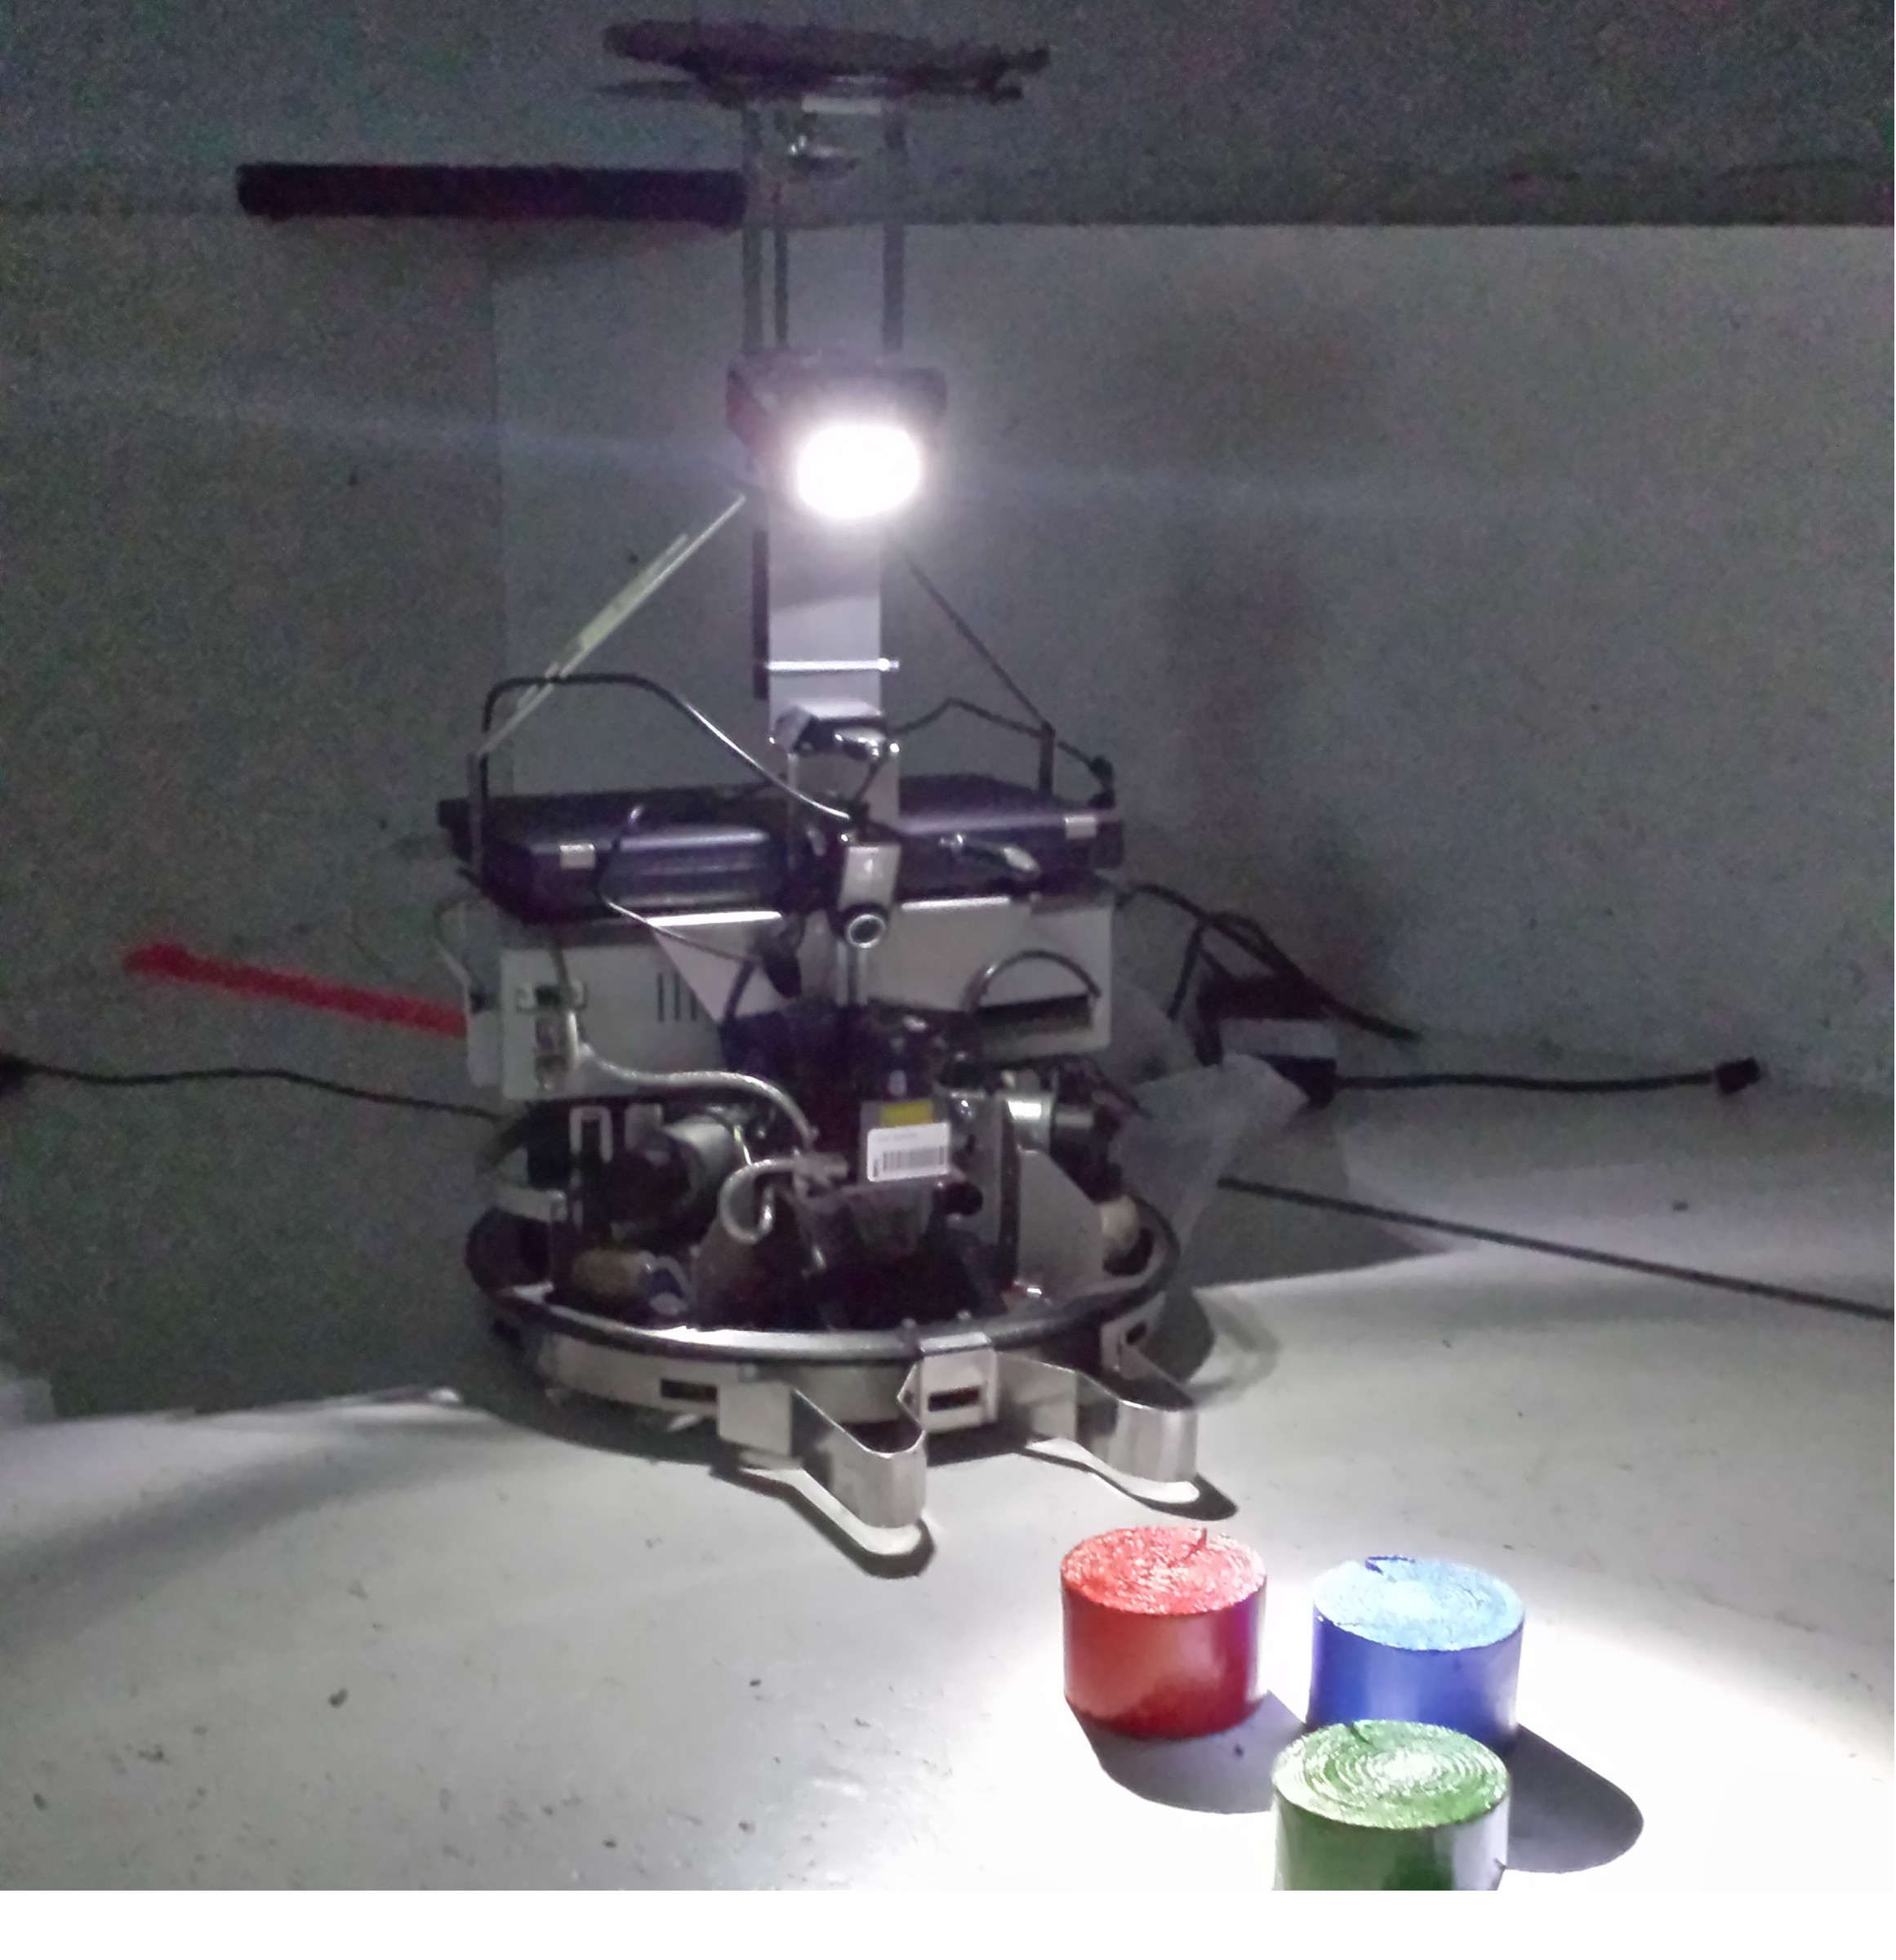
\includegraphics[width=\textwidth, height=\textwidth]{pics/hackathon_real_de}
    \caption{The Robotino is looking for colored pucks.}
    \label{fig:hackathon_real}
  \end{subfigure}
  \begin{subfigure}[b]{0.47\textwidth}
    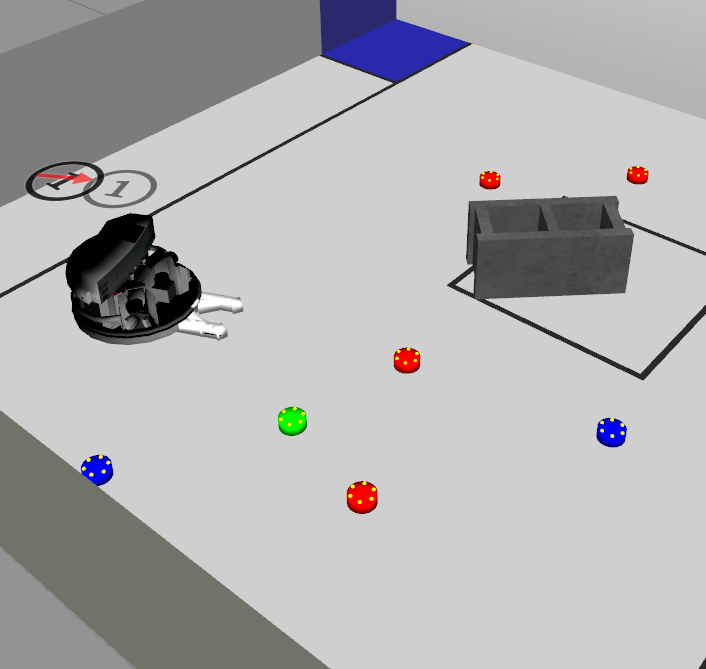
\includegraphics[width=\textwidth, height=\textwidth]{pics/hackathon_sim}
    \caption{Same scene in the simulation\\}
    \label{fig:hackathon_sim}
  \end{subfigure}
  \caption{Bonding Hackathon 2013: The Robotino has to find pucks with a webcam and bring them to a safe area.}
  \label{fig:hackathon}
\end{figure}
We successfully used our simulation in a Hackathon in November 2013. About 40 people participated in the Hackathon and used the simulation to develop a skill with Fawkes and Lua in a search and rescue scenario. The people had no previous experience with the simulator or our robot system. The event lasted one night including an introduction into developing skills for the Behavior Engine and was organized by Bonding\footnote{Bonding is a student association which organizes events to provide insights into the working life and contacts to companies looking for employees (\url{http://www.bonding.de}).} and Carologistics. The task was to find colored pucks with the Robotino in the dark and bring the pucks to a safe area. Figure~\ref{fig:hackathon_real} shows a Robotino doing this task. In addition to the equipment in LLSF, the Robotino holds a flashlight and a webcam looking downwards to detect pucks. The simulation was an essential part of the Hackathon for multiple reasons. There were about 40 participants, who worked in teams of two or three people, and only 4 available Robotinos and fields. Therefore, the simulation was necessary to provide the possibility of frequent testing and testing was important because the participants had no experience with Lua, the Robotino and the Behavior Engine. The scripts allowed easy and fast starting of the simulation and all needed components to operate the simulated Robotino. So, the participants did not need to know how to start Gazebo, ROS and Fawkes with additional plugins. Furthermore, the simulation provided a safe environment where no hardware could be damaged. The successful use of the simulation at the Hackathon also shows the capabilities of the simulation. Many teams primarily tested their code in the simulation and added only slight changes after testing on the real robot. This shows that the simulation is very similar to the real application. Feedback from some participants showed that the simulator is easy to use and runs with a high simulation speed close to real time even on the slow notebook provided at the Hackathon. We were able to increase the simulation speed because the Hackathon task did require less physical accuracy than the LLSF task because of less collisions between multiple puck and the wall. However, the graphical user interface of the simulator reacted more slowly than on faster computers because the provided notebooks had an old graphic card.\\
The use of the simulation at the Hackathon also showed that the simulation is extendable and easy to modify. The new approach to detect pucks with different colors works well with the webcam module developed for machine light detection and modifying the scripts and  models for the Robotino and the LLSF field with colored pucks and obstacles was easy and fast. We also deactivated the modules and plugins we did not need in the Hackathon to save performance.\\
The Hackathon was successful, most teams were able to develop a working skill which saved multiple pucks in the final competition on the real robot. Some teams performed very well and saved nearly all pucks.

\subsection{Limitations}
In this subsection, we describe the limitations of the simulation. First of all, a simulation cannot substitute testing with a real robot completely because the reality is too complex to simulate precisely. It is especially difficult to simulate realistic physics and graphics. Because of that, we were not able to appropriately simulate omni-directional wheels with realistic odometry errors and reflections on machine signal-lights which cause problems for machine light recognition. Furthermore, the available performance on current computers limits the number of simulated robots and sensor update rate and precision at a reasonable simulation speed and physical accuracy. Unfortunately, some limitations of the simulation of low level sensors and actuators also restrict the possibility to test components on a higher level with dependencies on these low level components. For example, we cannot test the reaction of our light-signal detection on reflections because we cannot simulate realistic reflections. A limitation of our automated simulation run is the human interaction in the multi-robot system. In LLSF, teams can remove misbehaving robots from the game and restart a robot a single time. This can only be done in the automated tests if a human is present all the time. As we show in this thesis, we were able to develop a useful and sufficiently realistic simulation despite all these limits.\\

\section{Multi-Robot Strategies}
\label{sec:multi_robot_strategies}
In this section, we evaluate our multi-robot system and the improvements we made with the simulation. This shows what the simulation can help to evaluate and where we have to improve our system in the future. We compare the improved system to the version at RoboCup 2013 in Eindhoven. As mentioned in section~\ref{sec:multi_agent_strategies}, we used two Robotinos, one with the $P_3$-role to produce $P_3$ pucks, which require only one production step, and one with the $P_1P_2$-role, which produces complex products. Unfortunately, the real performance in Eindhoven is not suitable for comparison with simulation runs because of the human interaction with misbehaving robots in the real game and less wrong perception results in the simulation. Furthermore, we also applied small improvements to the system that cause the system to perform better than in Eindhoven. Therefore, we rather use simulation runs with the same configuration as in Eindhoven as a basis for comparison.
\begin{figure}
  \centering
  \begin{tikzpicture}
    \begin{axis} [
          height=0.7\textwidth,
          width=\textwidth,
          xtick=data,
          xticklabels={$Eindhoven$,$P_1P_2$-$P_3$,$P_3$-$P_3$,$P_1P_2$-$P_3$-$R$,$P_1P_2$-$P_3$-$D$,$P_1$-$P_2$-$RD$},
          table/header=false,
          ylabel=Points,
          xlabel=Agent Configuration
        ]
        \addplot [box plot median] table {evaluation.dat};
        \addplot [box plot box] table {evaluation.dat};
        \addplot [box plot top whisker] table {evaluation.dat};
        \addplot [box plot bottom whisker] table {evaluation.dat};
    \end{axis}
  \end{tikzpicture}
  \caption{The box-plots show the amount of points reached in multiple LLSF simulation runs with two robots. \textit{Eindhoven} shows the real performance at the RoboCup 2013, all other results were simulated. The labeling marks used roles and improvements ($R$: recycling, $D$: dynamic role change). Each configuration was tested 10 to 15 times.}
  \label{fig:eval_two}
\end{figure}
Figure~\ref{fig:eval_two} shows the performances with two robots. The $R$ and $D$ at the end of the configuration name indicate if the configuration uses our recycling or dynamic role change improvement. We simulated 10 to 15 runs for each configuration. All experiments in the simulation have in common that there are more outliers with poor performance because we cannot restart misbehaving robots in the simulation. This also scatters the performance of single simulation runs because the amount of lost points caused by a misbehaving robot depends on the time when the misbehaving starts. Some of the most common causes for bad performances are shown in Figure~\ref{fig:fails}.
\begin{figure}
  \centering
  \begin{subfigure}[b]{0.38\textwidth}
    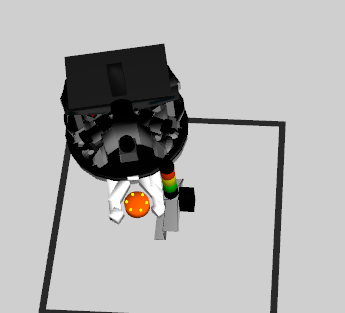
\includegraphics[width=\textwidth, height=\textwidth]{pics/bad_performance_eindhoven_no_reset}
    \caption{The Robotino wants to turn left, but cannot reach the target position because of the machine.}
    \label{fig:fails_stuck}
  \end{subfigure}
  \begin{subfigure}[b]{0.38\textwidth}
    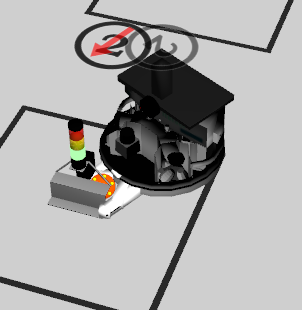
\includegraphics[width=\textwidth, height=\textwidth]{pics/wrong_local_bad_angle}
    \caption{Stuck Robotino after approaching the machine from an inappropriate angle}
    \label{fig:fails_angle}
  \end{subfigure}
  \begin{subfigure}[b]{0.38\textwidth}
    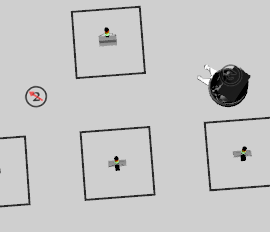
\includegraphics[width=\textwidth, height=\textwidth]{pics/p1_p2_wrong_localization_block_ins}
    \caption{The Robotino is wrongly localized and cannot reach the destination.}
    \label{fig:fails_localization}
  \end{subfigure}
  \begin{subfigure}[b]{0.38\textwidth}
    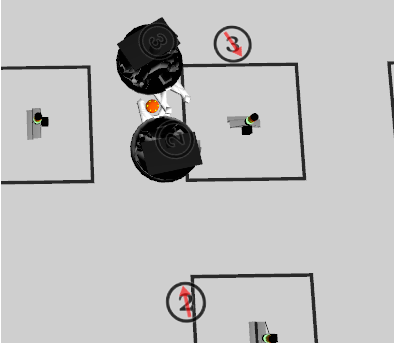
\includegraphics[width=\textwidth, height=\textwidth]{pics/crash_p3_p3_wrong_localization}
    \caption{Robotinos having troubles passing each other.}
    \label{fig:fails_passing}
  \end{subfigure}
  \caption{Failures and problems causing bad performance}
  \label{fig:fails}
\end{figure}
Figures~\ref{fig:fails_stuck} and~\ref{fig:fails_angle} show situations in which the Robotino gets stuck during low level movement. Often these situations block the robots the rest of the game because there is no timeout to detect that the robot is stuck or the recovery method is not able to solve the situation. These situations have a large impact on the performance of the system. The situations shown in Figure~\ref{fig:fails_localization} and~\ref{fig:fails_passing} happen during navigation. Often, such situations get solved, but it can take much time. These situations also can block the whole multi-robot system if one of the involved robots locks a position other robots need, too.\\
Because these problems limit the possibilities of the system and therefore the impact of agent improvements, good runs of different configurations are more meaningful when comparing different agents.\\
As we can see in Figure~\ref{fig:eval_two}, two $P_3$ agents perform better than one $P_1P_2$ and one $P_3$ agent. This is due to the fact that $P_3$ provides more points per production step and is less likely to fail because of the lower amount of steps needed to finish a $P_3$ puck. We did not use two $P_3$ agents at the RoboCup in Eindhoven although this would have been already possible but was untested at this time. We simply needed most of the testing time for components on a lower level. This again shows how useful the simulation is for evaluation.

\subsection{Dynamic Role Change}
We expected that the \textit{$P_1P_2$-$P_3$-$D$} configuration would performs 10 to 20 points better per run than the \textic{$P_1P_2$-$P_3$} configuration because after finishing the first complex product the $P_1P_2$ agent becomes a second $P_3$ agent. Surprisingly, the performance of $P_1P_2$-$P_3$-$D$ is not better than the performance of $P_1P_2$-$P_3$. The reconstructions of the simulated $P_1P_2$-$P_3$-$D$ runs show that a role change happens late and only rarely because it takes a large part of the game-time to finish the complex product and when the $P_1P_2$ agents gets stuck, it happens often in a way shown above and therefore the role change does not happen. The effects of the dynamic role change on the \textit{$P_1$-$P_2$-$RD$} configuration is similar. The statistics about the produced and delivered pucks show that the change worked in $30\%$ of the games and provided 10 to 30 additional points.\\
Overall the dynamic role change has potential that is limited by the slow production speed and situations in which the robot gets completely stuck.

\subsection{Recycling}
The \textit{$P_1P_2$-$P_3$-$R$} configuration mostly performs better than the $P_1P_2$-$P_3$ configuration. The statistics show that the $P_1P_2$ agent scores 5 to 10 additional points via recycling. The first 5 recycling points are scored early in the game after the $S_2$ production and further recycling points depend on the finished production of a complex product. The reconstructions of some simulation runs, especially with three robots, show that the recycling helps to avoid the bottleneck at the insertion area where robot get new $S_0$ pucks. However, Figure~\ref{fig:eval_two} shows that there are also a couple of games with a worse performance than $P_1P_2$-$P_3$. The reason is that the recycling step is more likely to fail than just getting a new $S_0$ puck. There are cases in which the Robotino gets stuck at a machine when trying to grep a consumed puck and in which the Robotino has problems with leaving the recycle machine. In no simulated game the recycling was necessary because of $S_0$ pucks running out of stock. This might change in the future if we can produce more and faster.

\subsection{Role Configurations for Three Agents}
To find a good role assignment for three robots and figure out the problems we need to tackle in the future, we compare several configurations here. Figure~\ref{fig:eval_three} shows the evaluation results with the configurations \textit{$P_1P_2$-$P_3$-$P_3$-$RD$}, \textit{$P_1$-$P_2$-$P_3$-$RD$} and \textit{$P_3$-$P_3$-$P_3$}.
\begin{figure}
  \centering
  \begin{tikzpicture}
    \begin{axis} [
          xtick=data,
          height=0.6\textwidth,
          width=\textwidth,
          xticklabels={$P_1P_2$-$P_3$-$P_3$-$RD$,$P_1$-$P_2$-$P_3$-$RD$,$P_3$-$P_3$-$P_3$},
          table/header=false,
          ylabel=Points
        ]
        \addplot [box plot median] table {evaluation_3.dat};
        \addplot [box plot box] table {evaluation_3.dat};
        \addplot [box plot top whisker] table {evaluation_3.dat};
        \addplot [box plot bottom whisker] table {evaluation_3.dat};
    \end{axis}
  \end{tikzpicture}
  \caption{The box-plots show the amount of points reached in multiple LLSF simulation runs with three robots. The labeling and test population is equivalent to Figure~\ref{fig:eval_two}.}
  \label{fig:eval_three}
\end{figure}
Surprisingly, no configurations with three robots performs better than a similar configuration with two robots. The reasons can easily be seen in some reconstructions. First, using three robots lead to significantly more navigation conflicts, such as in Figure~\ref{fig:fails_passing}, than using two robots. This often also effects the third robot when it has to pass the other two robots or it needs a resources that is locked by another robot. Second, the bottleneck of the current approach, which is the single point for getting new pucks, affects three robots more than two. Therefore, robots often have to wait until for other robots. Third, the failure of single robots remains a big problem. On the one hand, there are two robots left if one fails, but on the other hand a failing robot that locked an important resource still blocks the whole system.




\chapter{Summery and Future Work}
\label{cha:summery_and_future_work}

This is the conclusion.


%reenable empty pages before chapter
\let\cleardoublepage\cleardoublepage

\newpage

\bibliographystyle{plain}
\bibliography{references}

\end{document}
